\documentclass[11pt,letterpaper]{article}

\usepackage[margin=1in]{geometry}
\usepackage{booktabs}
\usepackage{graphicx}
\usepackage{caption}
\usepackage{amsmath}
\usepackage{hyperref}
\usepackage{parskip}
\usepackage{microtype}
\usepackage{siunitx}

\sisetup{separate-uncertainty=true}

\title{SHS Lab Test --- 2026-05-28\\[0.4ex]
       \large Clark South Ballast Tank, WHOI}
\author{Yu Gao, Emerson Hasbrouck, Tom Farrar, Simon de Szoeke, Steven Jayne, and Alexander Ekholm}
\date{2026-05-28 (data through 2026-05-29 \textasciitilde11:10 UTC)}

\begin{document}
\maketitle
\hrule\bigskip

% ─────────────────────────────────────────────────────────────────────────────
\section{Setup}

Six dunk cycles in the Clark South saltwater ballast tank (30--32\,PSU) at
WHOI. A fan provided steady airflow to the WXT520 head throughout.

\begin{figure}[htbp]
  \centering
  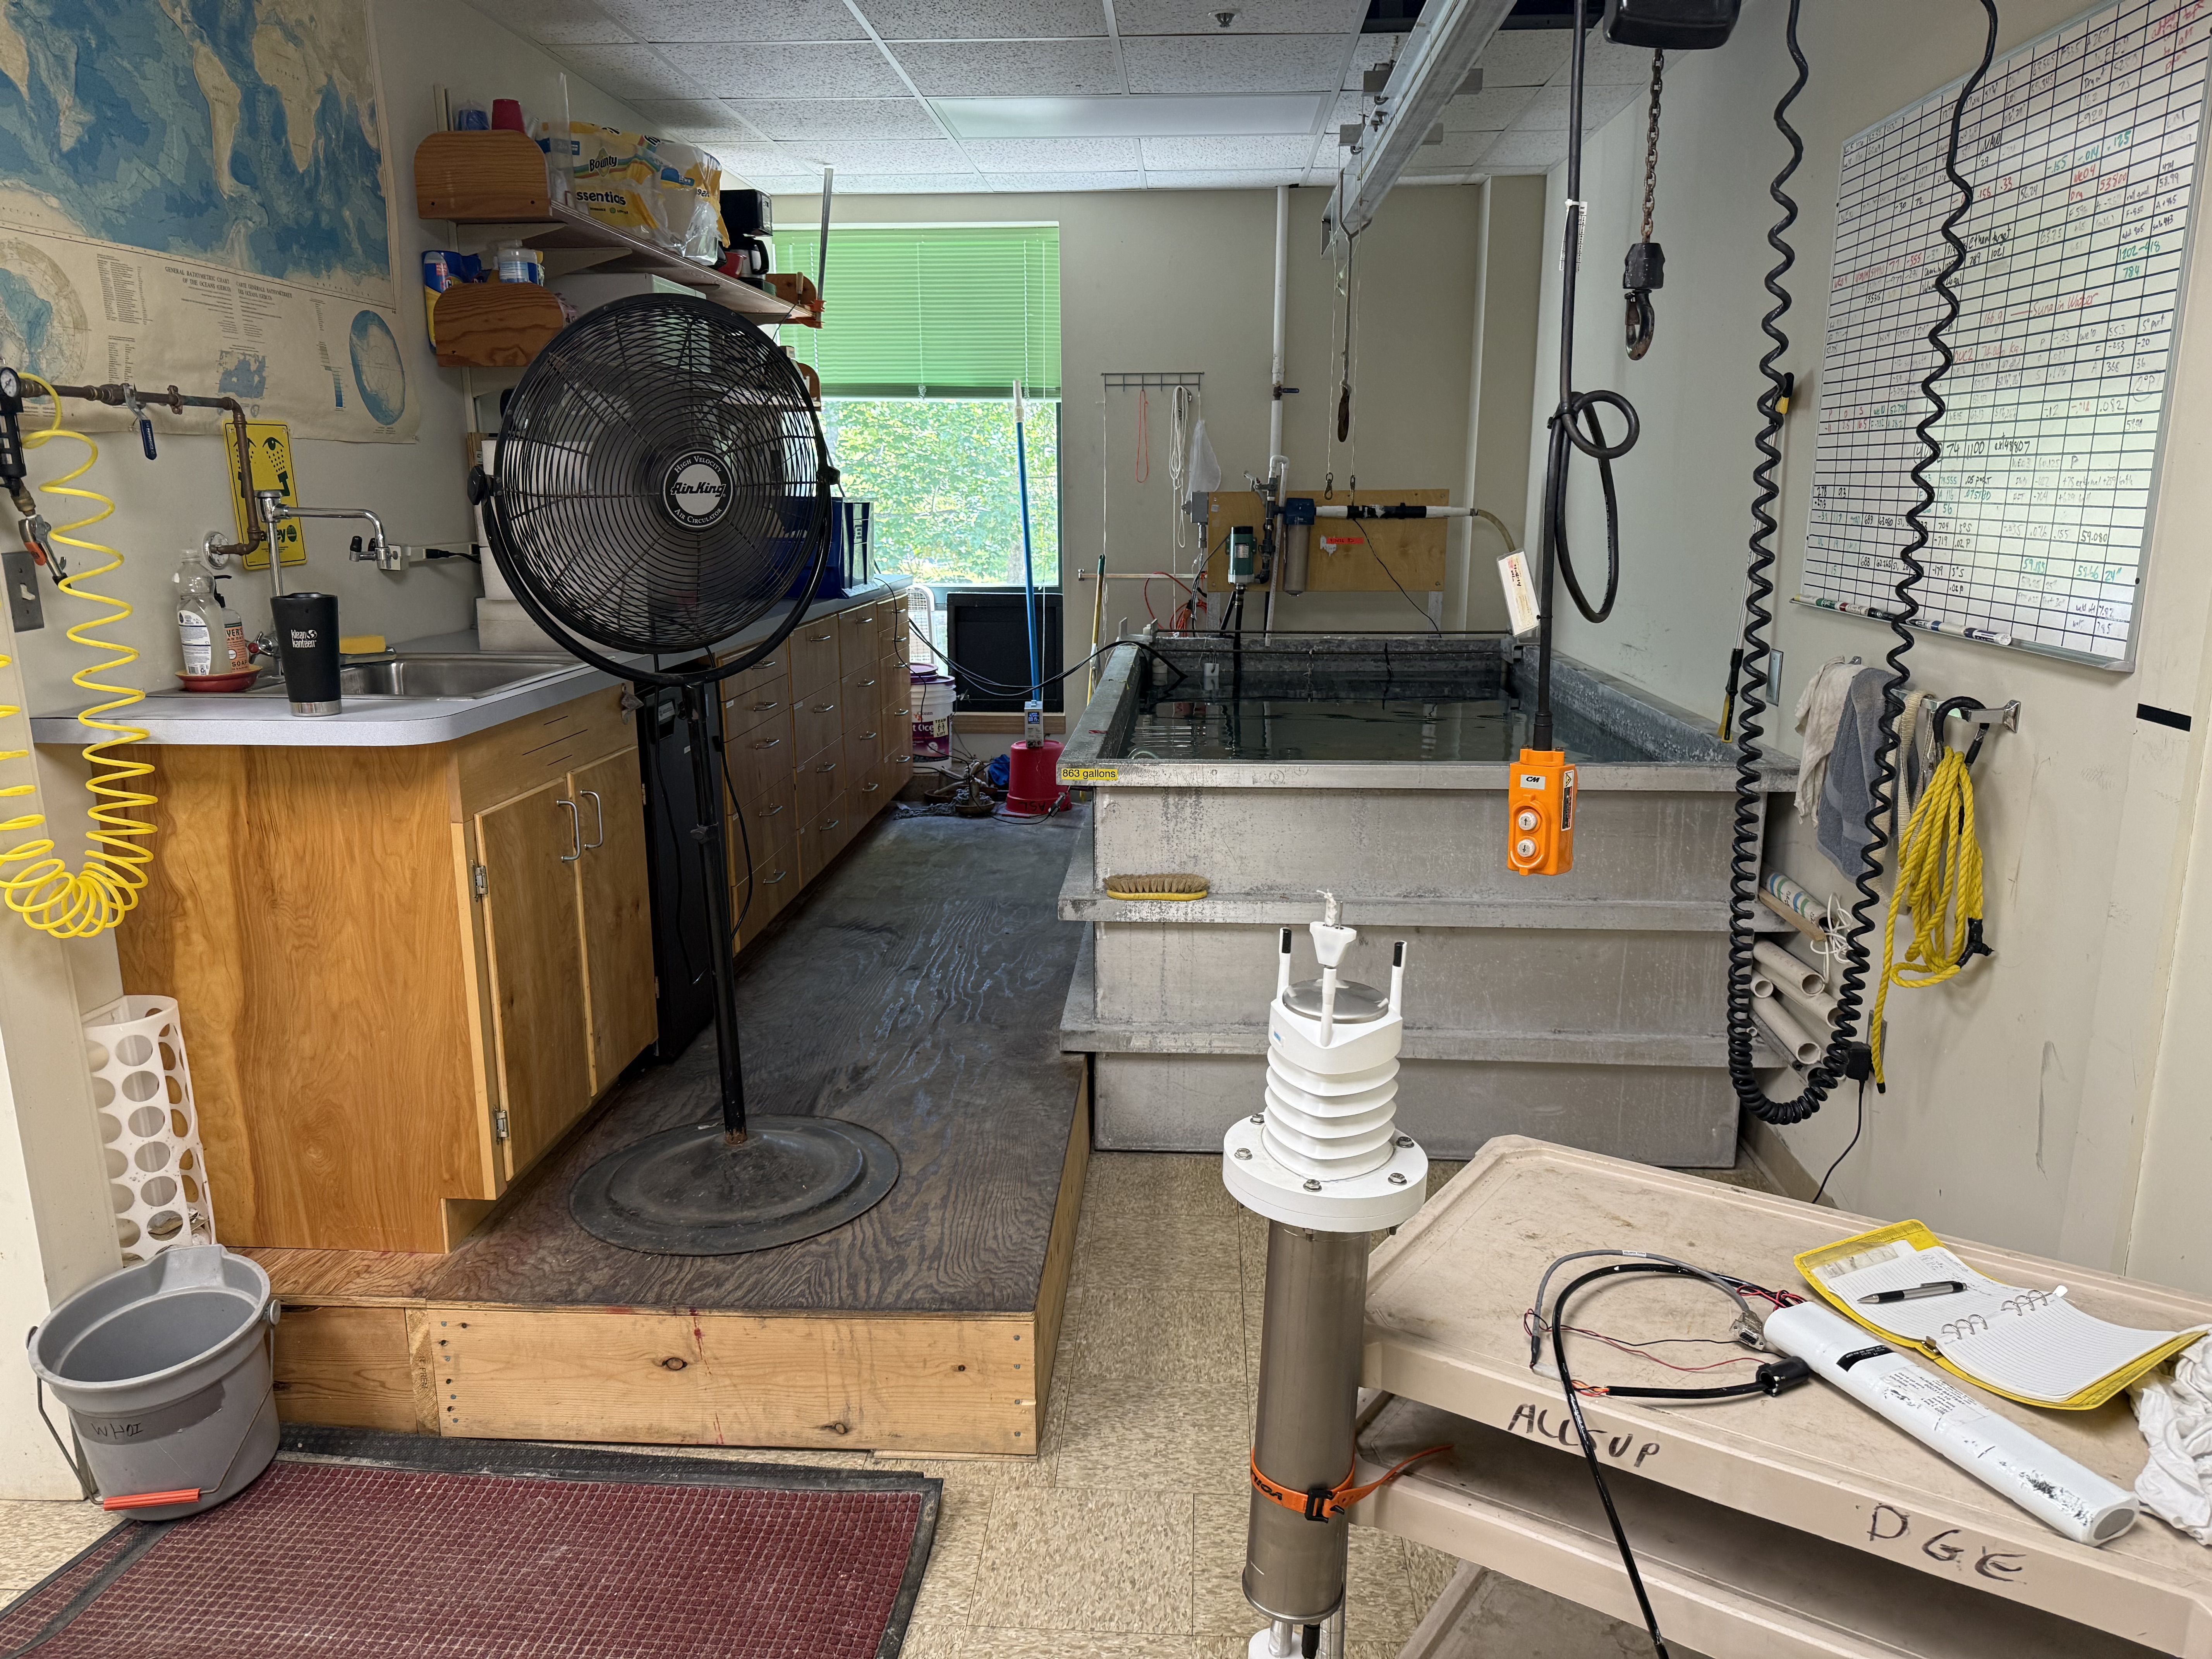
\includegraphics[width=0.72\linewidth]{../../data/20260528Lab/lab_environment.jpeg}
  \caption{Clark South ballast tank.  Fan and WXT520 visible at left.}
  \label{fig:lab_env}
\end{figure}

\begin{center}
\begin{tabular}{lll}
\toprule
Instrument & ID & Rate \\
\midrule
RBRduo3 T.T (dry/wet bulb) & SN 233860 & 3 s \\
Vaisala WXT520 (met) & ASWXT203 & 1 min \\
Seabird GPCTD (tank reference) & --- & 1 Hz \\
\bottomrule
\end{tabular}
\end{center}

\medskip
\begin{minipage}[t]{0.48\linewidth}
\begin{center}
\textbf{Event log (UTC, 2026-05-28)}\\[4pt]
\begin{tabular}{cccc}
\toprule
Cycle & IN & OUT & Duration \\
\midrule
IN-1 & 13:11 & 13:27 & 16 min \\
IN-2 & 13:56 & 14:01 &  5 min \\
IN-3 & 14:56 & 15:01 &  5 min \\
IN-4 & 15:42 & 15:49 &  7 min \\
IN-5 & 16:30 & 16:34 &  4 min \\
IN-6 & 18:30 & 18:50 & 20 min \\
\bottomrule
\end{tabular}
\end{center}
Instruments on at 13:08; recovered 2026-05-29 \textasciitilde11:10 UTC.
\end{minipage}\hfill
\begin{minipage}[t]{0.48\linewidth}
\begin{center}
\textbf{Ambient conditions (WXT, 13:08--19:00 UTC)}\\[4pt]
\begin{tabular}{lSS}
\toprule
Variable & {Mean} & {Std} \\
\midrule
Air temperature (\si{\degreeCelsius}) & 18.17 & 0.15 \\
Relative humidity (\%)               & 64.4  & 0.8  \\
Barometric pressure (mbar)           & 1006.89 & 0.12 \\
Wind speed (scalar mean, m/s)        & 1.81  & {---}  \\
\bottomrule
\end{tabular}
\end{center}
\end{minipage}

% ─────────────────────────────────────────────────────────────────────────────
\section{Humidity: WXT520 vs.\ psychrometric}

\begin{figure}[htbp]
  \centering
  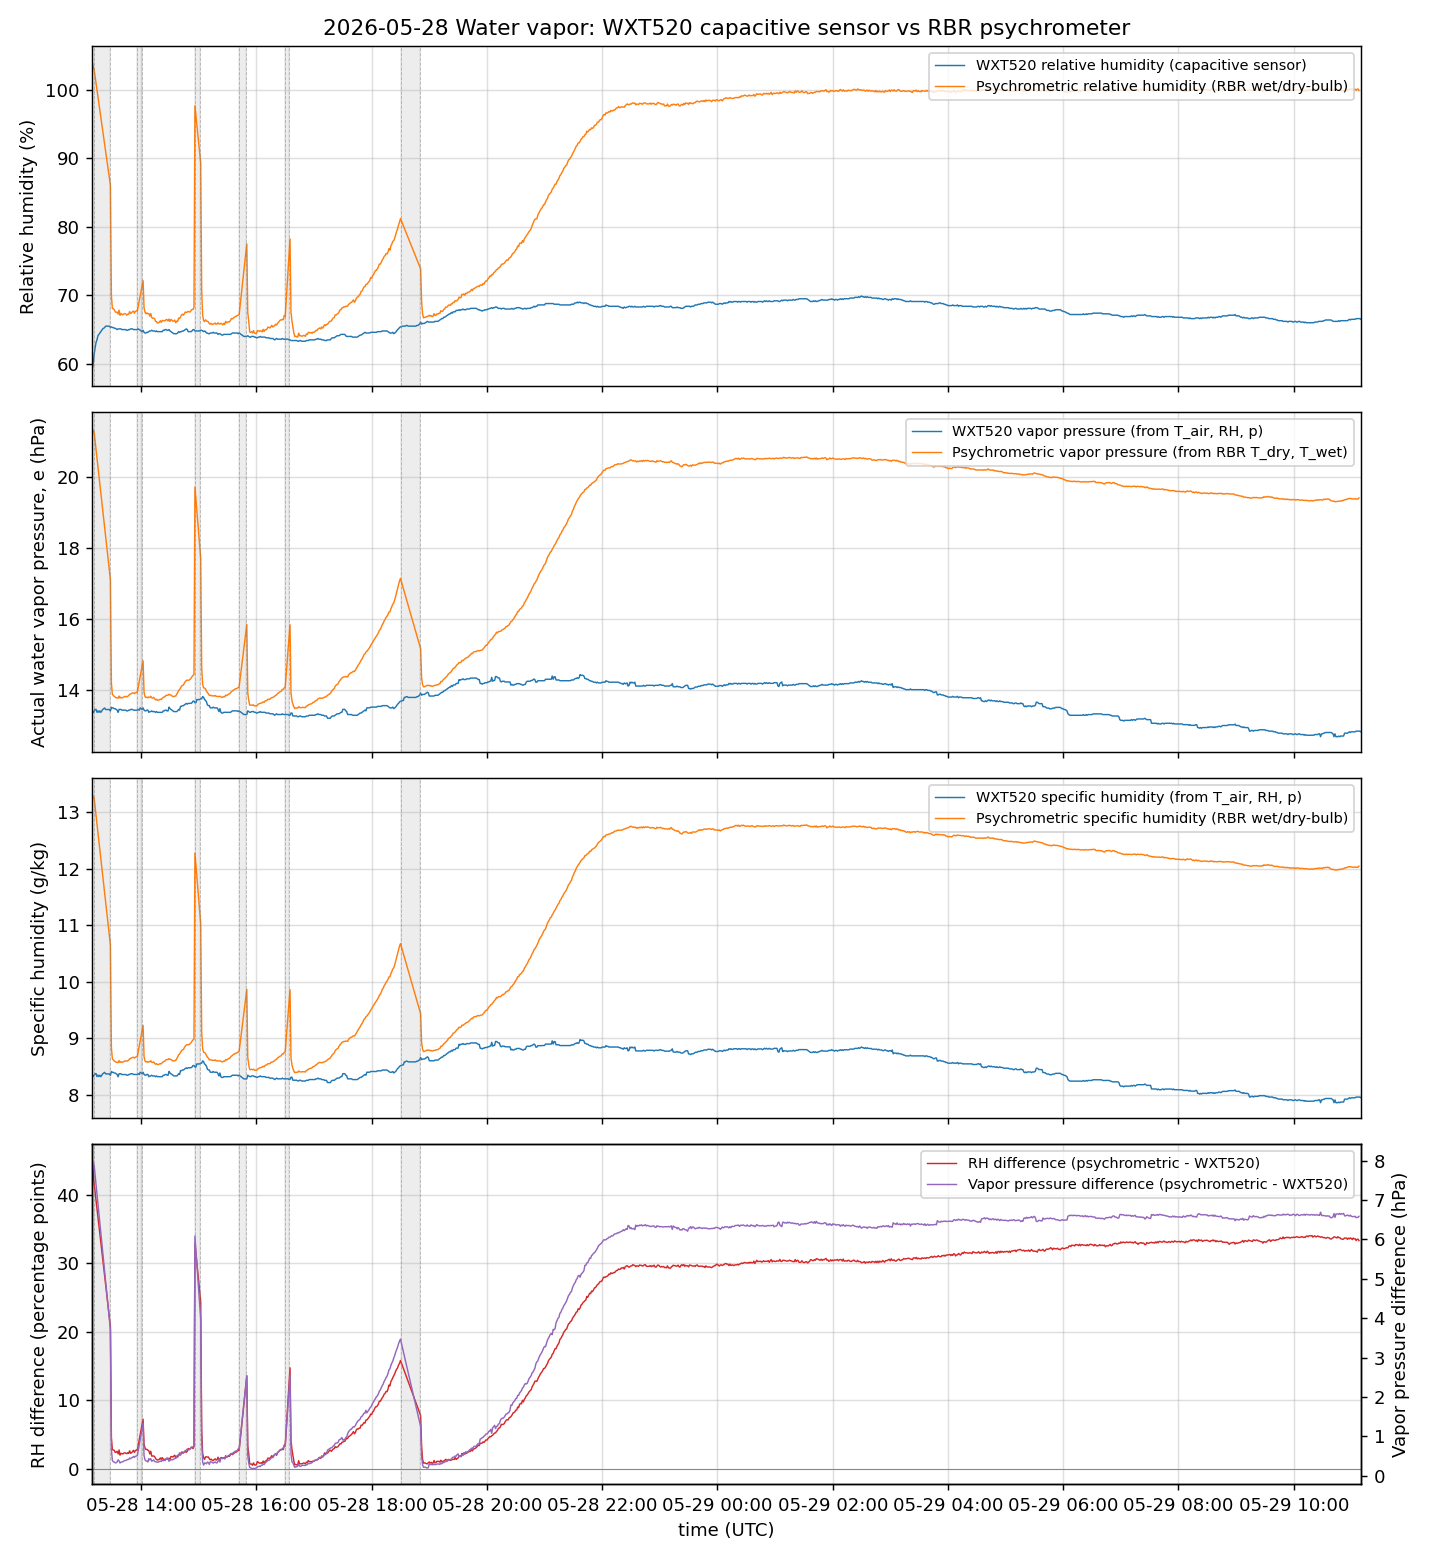
\includegraphics[width=\linewidth]{../../img/Lab20260528/Lab20260528_WXT_vs_psychrometric_humidity.png}
  \caption{Head-to-head comparison of the WXT520 capacitive humidity sensor
           against the RBR psychrometric calculation (wet/dry-bulb).
           Grey bands mark the six in-water periods.
           \textbf{Top:} relative humidity.
           \textbf{Middle two:} actual vapor pressure and specific humidity.
           \textbf{Bottom:} signed differences (psychrometric $-$ WXT520).}
  \label{fig:humidity}
\end{figure}

\begin{itemize}
  \item \textbf{During active test (13:08--18:50 UTC):} The two methods agree
    well at $\sim$64\,\% RH in air, with short spikes during each dunk as the
    wet bulb equilibrates with the saltwater.
  \item \textbf{Overnight (after IN-6):} The psychrometric RH rises to
    $\sim$100\,\% because the wick remained wet after the last dunk and the
    sensor was left in air overnight.  WXT520 stays stable at
    $\sim$65--68\,\%.  This is an artefact of the test procedure, not a sensor
    fault.
  \item \textbf{Residual offset:} Once the wick is saturated,
    psychrometric RH overshoots WXT by $\sim$4\,pct-pt
    ($\Delta e \approx +0.8$\,hPa) -- likely a small wick-induced evaporative
    enhancement.  To be monitored in future tests.
  \item \textbf{Action item:} A live WXT display during the test would give
    immediate feedback on wick state (per Simon's suggestion).
\end{itemize}

% ─────────────────────────────────────────────────────────────────────────────
\section{Temperature and sensor response}

\subsection*{SHS vs.\ in-tank GPCTD reference}

\begin{figure}[htbp]
  \centering
  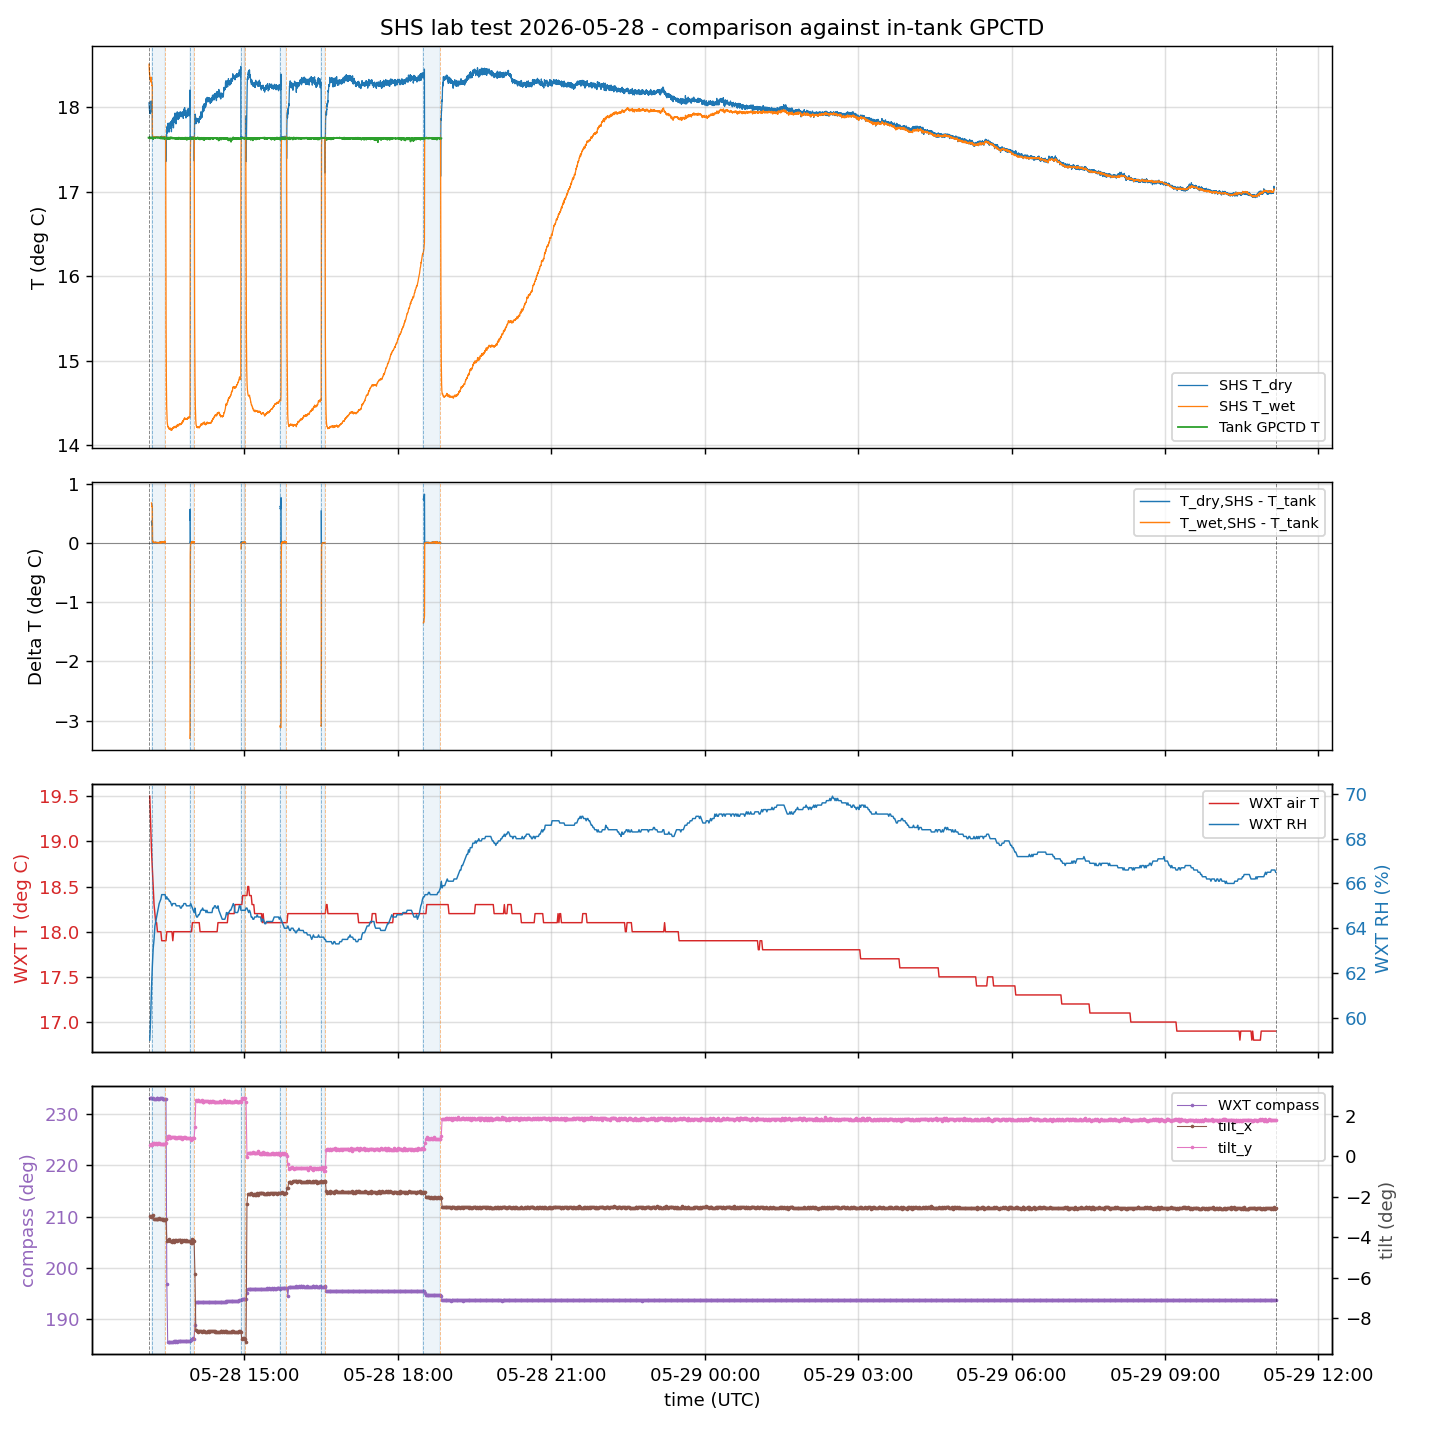
\includegraphics[width=\linewidth]{../../img/Lab20260528/Lab20260528_SHS_vs_tank.png}
  \caption{SHS dry/wet-bulb temperatures and GPCTD tank reference.
           \textbf{Top:} absolute temperatures.
           \textbf{Second:} $\Delta T$ (SHS $-$ tank), in-water periods only.
           \textbf{Third:} WXT air temperature and RH.
           \textbf{Bottom:} WXT compass and tilt (sensor attitude diagnostic).
           Blue bands: in-water periods.}
  \label{fig:vs_tank}
\end{figure}

$T_\text{wet}$ approaches tank temperature during each dunk;
$T_\text{dry}$ stays near ambient due to its larger thermal mass.
Compass and tilt are stable throughout, confirming no sensor movement.

\subsection*{Response-time fits (OUT events)}

\textbf{Method.}
An exponential model $y(t) = A + B\,e^{-t/\tau}$ is fitted by nonlinear least
squares to $T_\text{dry}$, $T_\text{wet}$, depression ($T_d - T_w$), and
psychrometric RH over a window from each OUT time to
$\min(\text{OUT}+25\,\text{min},\,\text{next IN})$.
$\tau$ is the $e$-folding recovery time.

\begin{center}
\begin{tabular}{lrrrr}
\toprule
OUT & $\tau_{T_d}$ (s) & $\tau_{T_w}$ (s) & $\tau_\text{dep}$ (s)
    & $\tau_\text{RH}$ (s) \\
\midrule
13:27 & 389  & 51 & 58 & 56 \\
14:01 & 1475$^*$ & 29 & 31 & 30 \\
15:01 &  74  & 61 & 65 & 64 \\
15:49 & 130  & 42 & 51 & 48 \\
16:34 & 139  & 41 & 54 & 51 \\
18:50 &  67  & 27 & 35 & 33 \\
\midrule
Median & 134 & 42 & 53 & 50 \\
\bottomrule
\end{tabular}

\smallskip{\footnotesize $^*$ window capped at 25 min; fit unreliable.}
\end{center}

\begin{figure}[htbp]
  \centering
  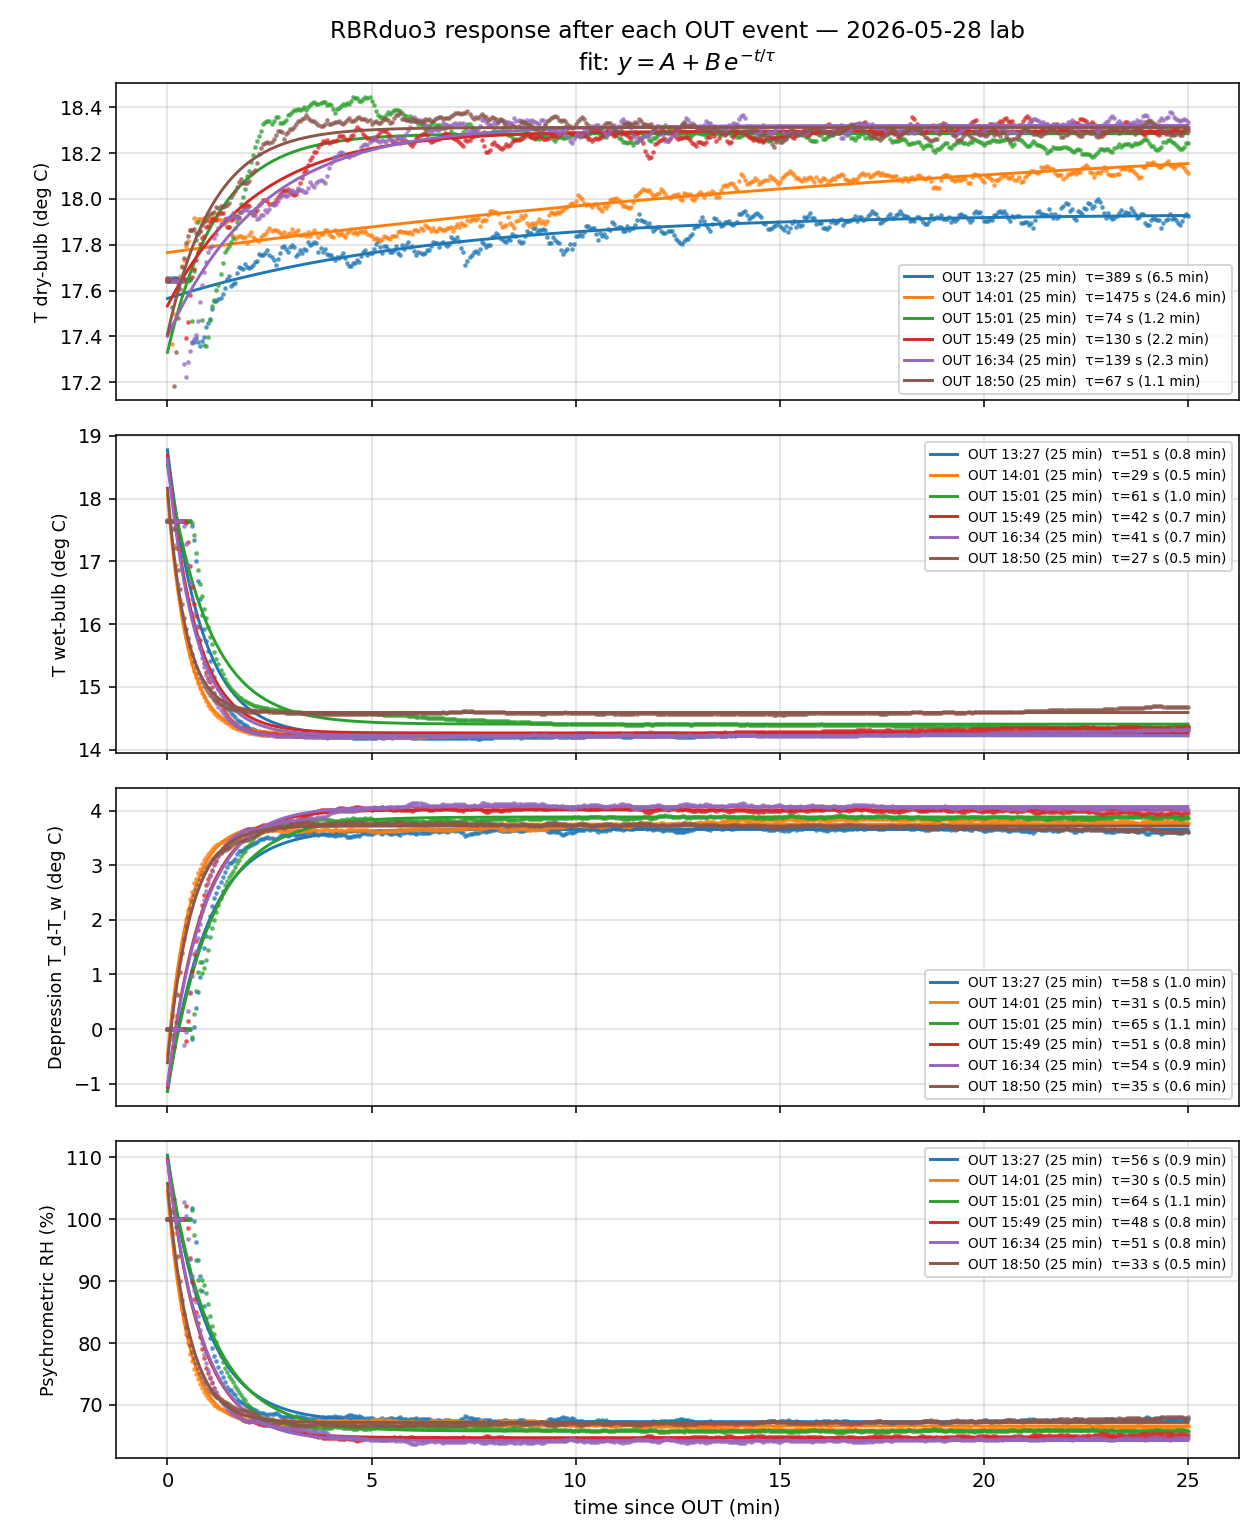
\includegraphics[width=\linewidth]{../../img/Lab20260528/Lab20260528_response_time.png}
  \caption{Exponential recovery fits for all six OUT events.}
  \label{fig:response_time}
\end{figure}

$T_\text{wet}$, depression, and RH recover in $\sim$30--65\,s.
$T_\text{dry}$ is the slow component (median $\tau \approx 134$\,s);
psychrometric RH inherits this when computed through $T_\text{dry}$.

\subsection*{Wet-bulb cooling (IN events)}

\begin{figure}[htbp]
  \centering
  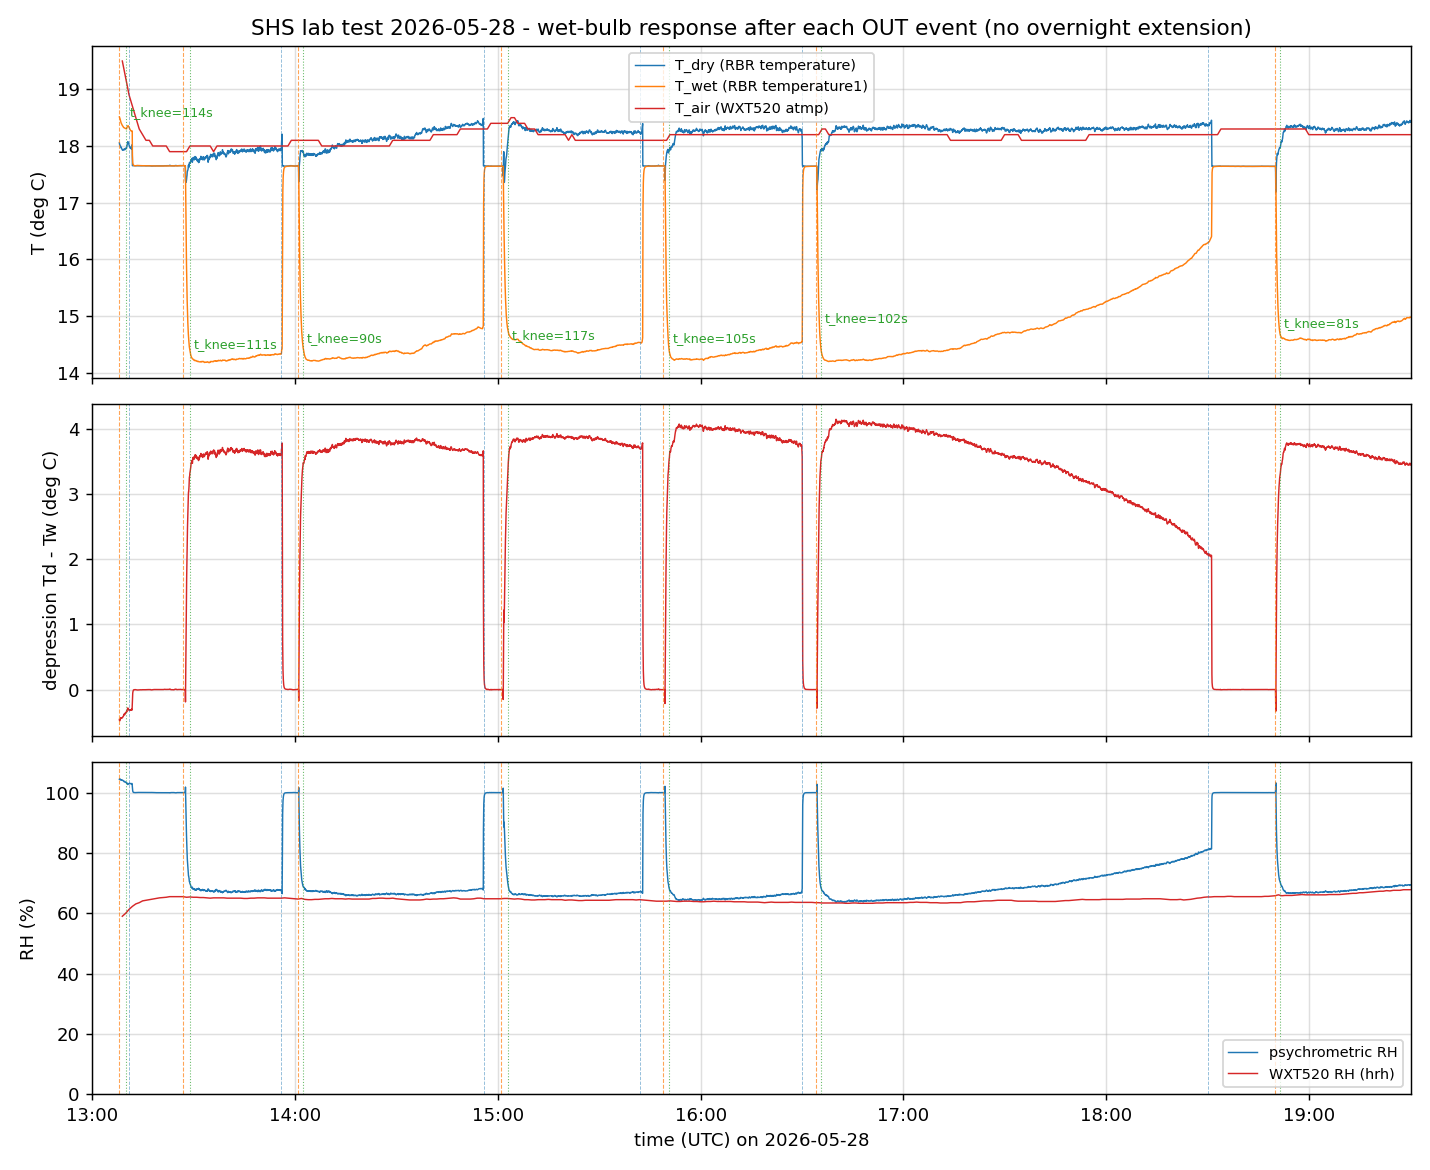
\includegraphics[width=\linewidth]{../../img/Lab20260528/Lab20260528_temp_drops.png}
  \caption{Wet-bulb cooling for each IN event.  Orange dashed: OUT time.}
  \label{fig:temp_drops}
\end{figure}

$T_\text{wet}$ peaks in cooling rate at $\sim$20--50\,s after submersion and
plateaus near tank temperature within $\sim$1\,min.

% ─────────────────────────────────────────────────────────────────────────────
\section{Wind}

\begin{figure}[htbp]
  \centering
  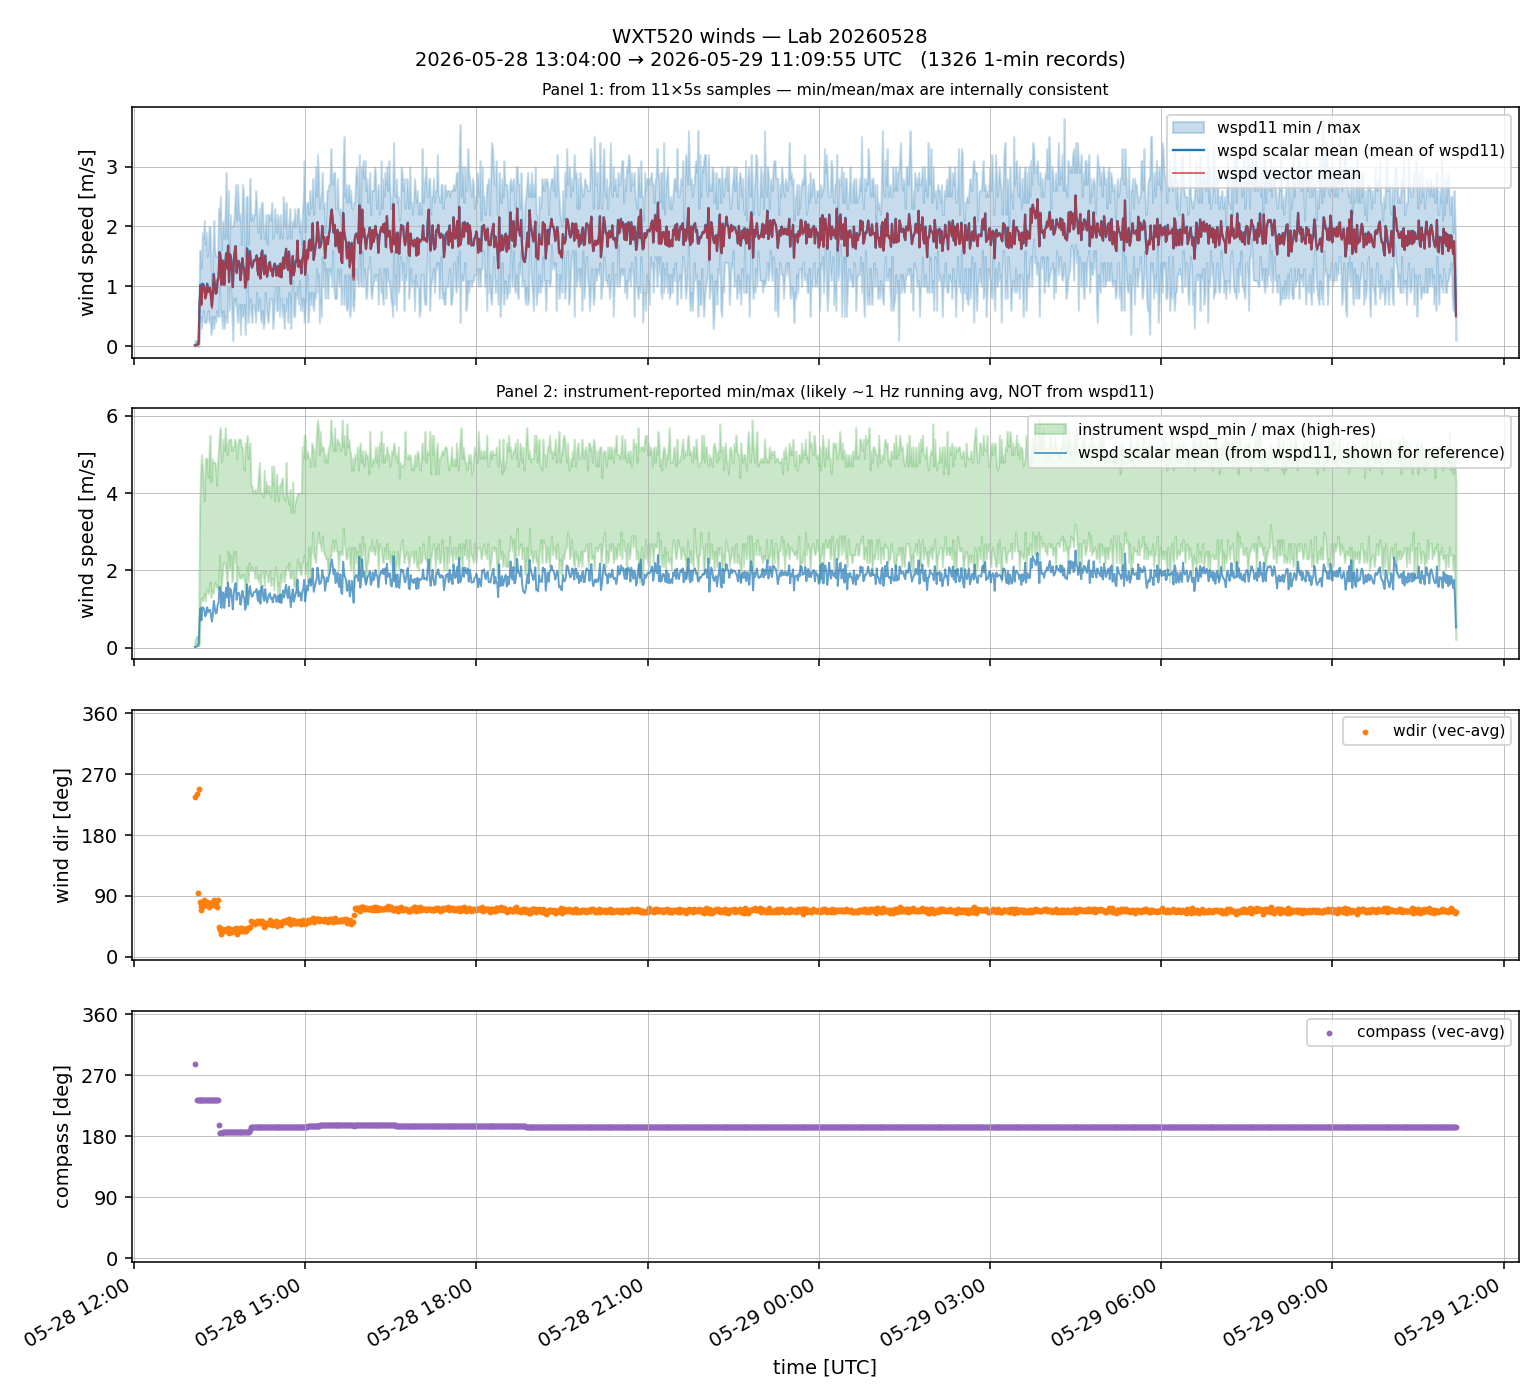
\includegraphics[width=\linewidth]{../../img/Lab20260528/WXT_wind_minmax_20260528.png}
  \caption{WXT520 wind over full deployment.
           \textbf{Top:} shaded band = min/max of \texttt{wspd11}
           (11 five-second samples/min); blue = scalar mean; red = vector mean.
           \textbf{Middle:} instrument-reported \texttt{wspd\_min}/\texttt{wspd\_max}
           (different population --- see text).
           \textbf{Bottom two:} wind direction and compass.}
  \label{fig:wind}
\end{figure}

Mean wind speed $\approx$1.8\,m/s (fan); compass stable at
$\sim$195\si{\degree}.

\textbf{Note on \texttt{wspd\_min}/\texttt{wspd\_max}:}
These fields originate from the WXT520's native serial output fields \texttt{Sn}
(speed minimum) and \texttt{Sx} (speed maximum).  The ASIMET GILWND45 front-end
board passes them through unchanged via a direct \texttt{aR1} relay --- it
applies no accumulation logic of its own
(\url{https://uop.whoi.edu/UOPinstruments/frodo/asimet/wxt520ifcmnd.html}).
The exact averaging window used by the WXT520 internally for \texttt{Sn}/\texttt{Sx}
versus \texttt{Sm} is configurable and documented only in the Vaisala WXT520
user manual, which has not yet been consulted.
Because \texttt{wspd\_min} exceeds \texttt{mean(wspd11)} in 99\,\% of records,
the two quantities are clearly not from the same population.
All reported wind statistics in this report use \texttt{wspd11} directly.

% ─────────────────────────────────────────────────────────────────────────────
\section{Next steps}

\begin{enumerate}
  \item \textbf{Consult Vaisala WXT520 user manual.}
    Determine the exact accumulation window for \texttt{Sn}/\texttt{Sx}
    (minimum/maximum wind speed) vs.\ \texttt{Sm} (mean), and confirm whether
    the ASIMET deployment uses the default WXT520 configuration.
    This will fully resolve the \texttt{wspd\_min} $>$ \texttt{mean(wspd11)}
    discrepancy.

  \item \textbf{Pre-wet the wick before each test.}
    IN-1 through IN-3 showed undersaturation.  Soak the wick in fresh water
    for $\sim$5\,min before the start of each test session.

  \item \textbf{Add a live WXT display during tests.}
    A real-time readout of WXT RH and air temperature would give immediate
    feedback on wick saturation and ambient stability (per Simon's suggestion).

  \item \textbf{Repeat the overnight soak intentionally.}
    The post-IN-6 overnight data showed psychrometric RH rising to
    $\sim$100\,\% as the wet wick dried in air.  A controlled version of this
    (sensor left in known-humidity air overnight) would provide a cleaner
    characterisation of wick drying rate and long-term psychrometric drift.

  \item \textbf{Quantify the $\sim$4\,pct-pt psychrometric offset.}
    Once wick saturation is reliable (IN-4 onward), the psychrometric RH
    overshoots WXT by $\sim$4\,pct-pt.  Repeat tests with a calibrated
    reference hygrometer to determine whether this is a systematic wick bias,
    a WXT calibration offset, or a pressure/temperature correction issue.
\end{enumerate}

\end{document}


\sisetup{separate-uncertainty=true}

\title{SHS Lab Test --- 2026-05-28\\[0.4ex]
       \large Clark South Ballast Tank, WHOI}
\author{E.\ G.\ Hayden}
\date{2026-05-28 (data through 2026-05-29 \textasciitilde11:10 UTC)}

\begin{document}
\maketitle
\hrule\bigskip

% ─────────────────────────────────────────────────────────────────────────────
\section{Setup}

Six dunk cycles were performed in the Clark South saltwater ballast tank
(30--32\,PSU) at WHOI.  A fan provided steady airflow to the WXT520 head.

\begin{center}
\begin{tabular}{lll}
\toprule
Instrument & ID & Rate \\
\midrule
RBRduo3 T.T (dry/wet bulb) & SN 233860 & 3 s \\
Vaisala WXT520 (met) & ASWXT203 & 1 min \\
Seabird GPCTD (tank reference) & --- & 1 Hz \\
\bottomrule
\end{tabular}
\end{center}

\begin{figure}[htbp]
  \centering
  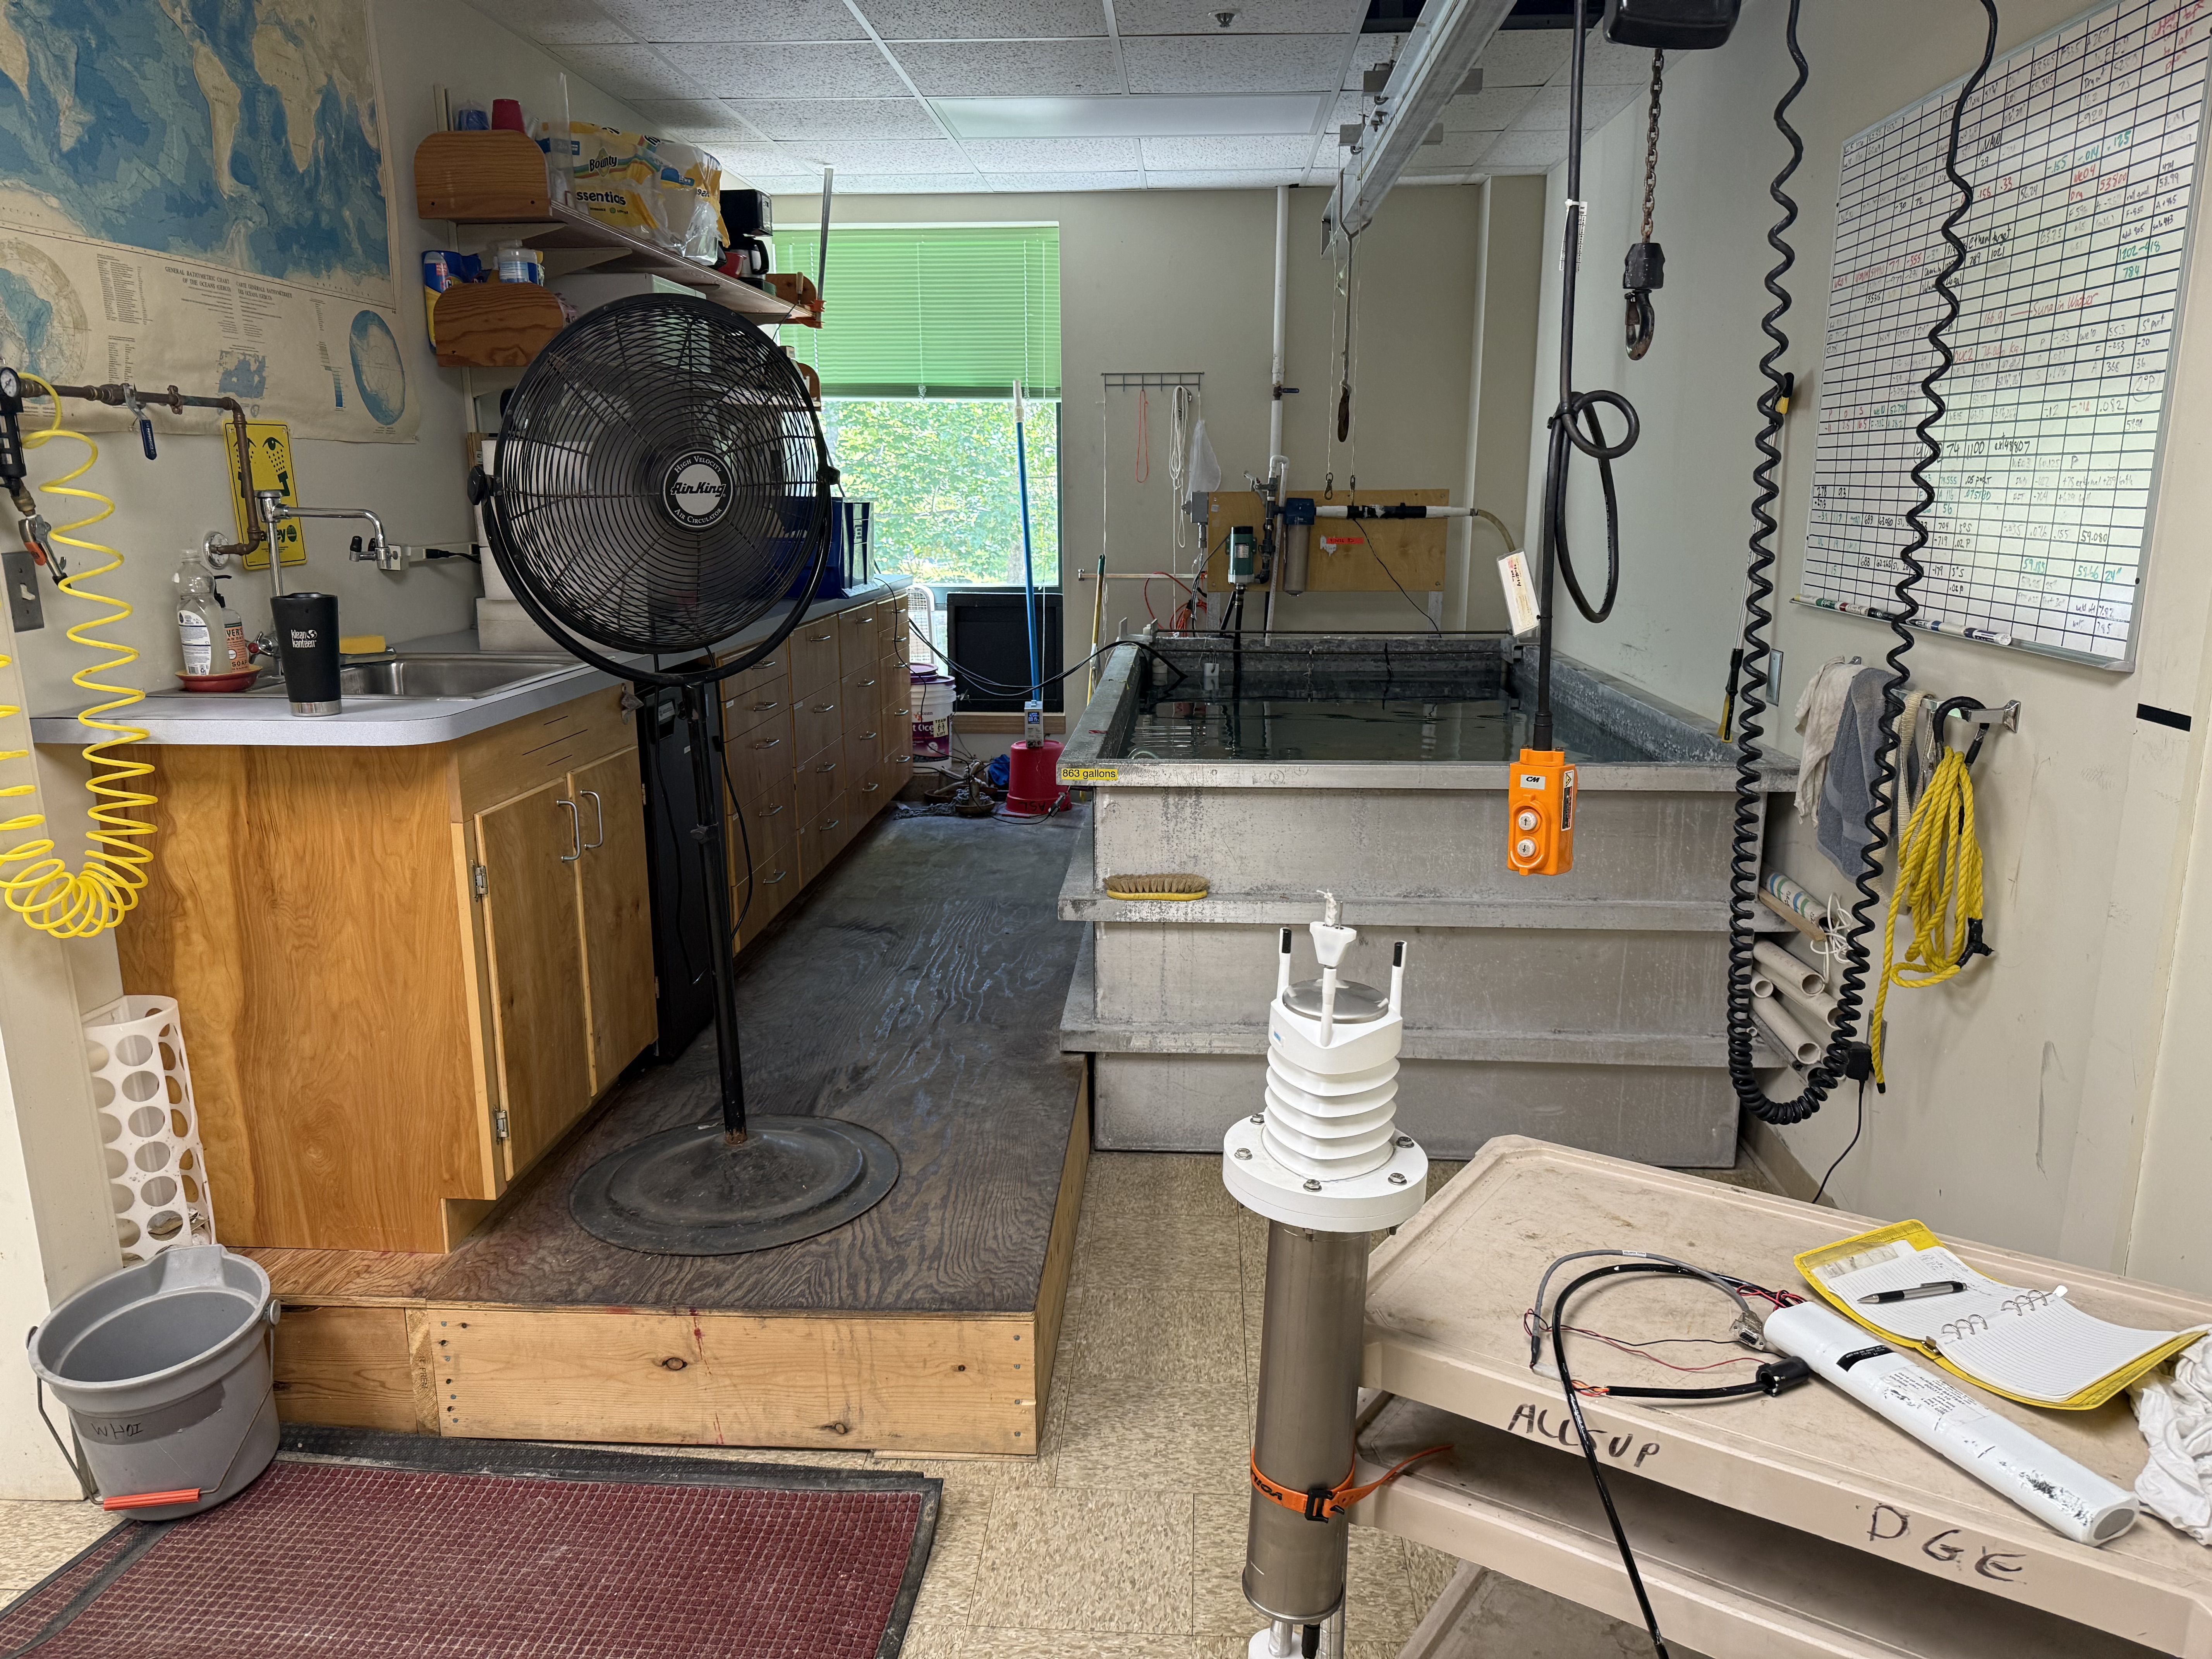
\includegraphics[width=0.75\linewidth]{../../data/20260528Lab/lab_environment.jpeg}
  \caption{Clark South ballast tank.  Fan and WXT520 visible at left.}
  \label{fig:lab_env}
\end{figure}

% ─────────────────────────────────────────────────────────────────────────────
\section{Event log (UTC)}

\begin{center}
\begin{tabular}{cccc}
\toprule
Cycle & IN & OUT & Duration \\
\midrule
IN-1 & 13:11 & 13:27 & 16 min \\
IN-2 & 13:56 & 14:01 &  5 min \\
IN-3 & 14:56 & 15:01 &  5 min \\
IN-4 & 15:42 & 15:49 &  7 min \\
IN-5 & 16:30 & 16:34 &  4 min \\
IN-6 & 18:30 & 18:50 & 20 min \\
\bottomrule
\end{tabular}
\end{center}

Instruments on, fan on at 13:08.  Recovered 2026-05-29 \textasciitilde11:10 UTC.

% ─────────────────────────────────────────────────────────────────────────────
\section{Ambient conditions (WXT520, 13:08--19:00 UTC)}

\begin{center}
\begin{tabular}{lSS}
\toprule
Variable & {Mean} & {Std} \\
\midrule
Air temperature (\si{\degreeCelsius}) & 18.17 & 0.15 \\
Relative humidity (\%)               & 64.4  & 0.8  \\
Barometric pressure (mbar)           & 1006.89 & 0.12 \\
Wind speed (m/s, scalar mean)        & 1.81  & {---}  \\
\bottomrule
\end{tabular}
\end{center}

% ─────────────────────────────────────────────────────────────────────────────
% \section{Full-duration overview}

\begin{figure}[htbp]
  \centering
  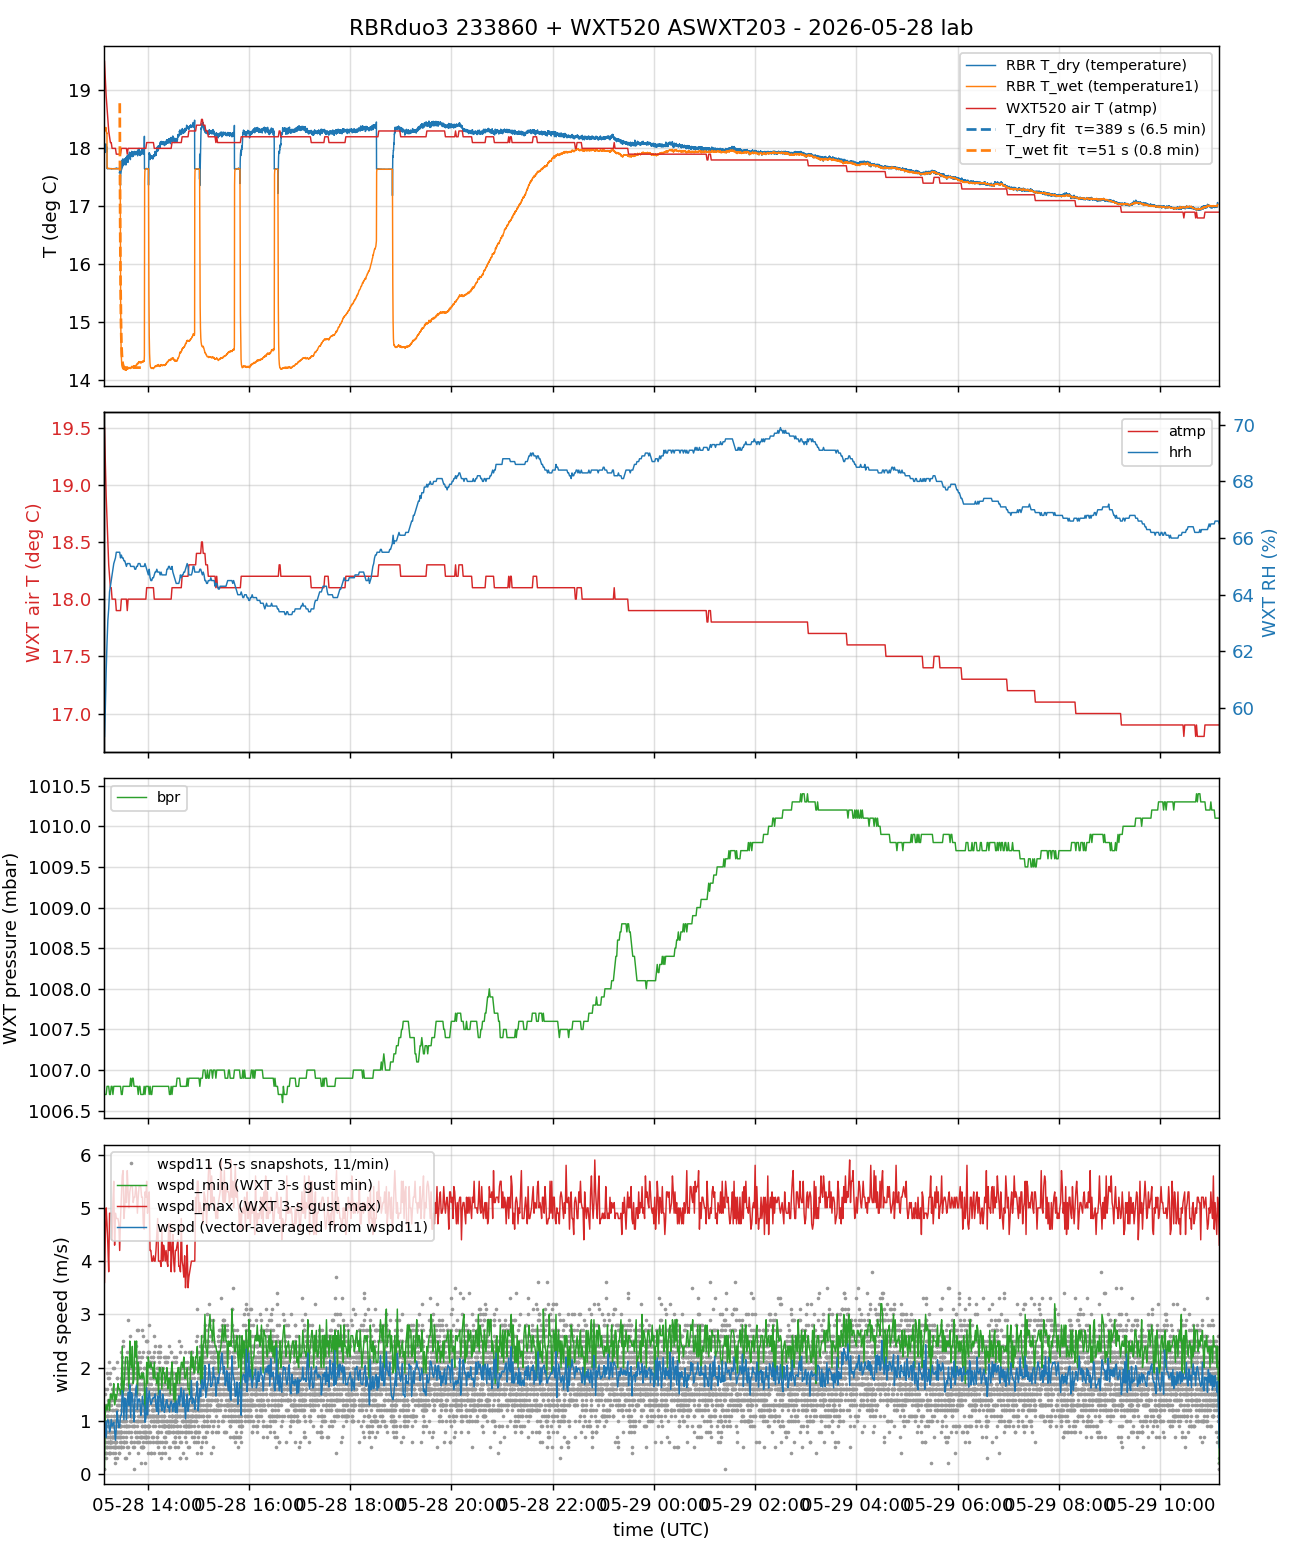
\includegraphics[width=\linewidth] {../../data/20260528Lab/Lab20260528_RBR_WXT_timeseries.png}
  \caption{Full time series.  RBR dry/wet-bulb, WXT air temperature and RH,
           barometric pressure, and wind speed.  $T_\text{wet}$ dips at each
           dunk; all other variables are stable throughout.}
  \label{fig:timeseries}
\end{figure}

% ─────────────────────────────────────────────────────────────────────────────
\section{Psychrometric RH vs.\ WXT reference}

\begin{figure}[htbp]
  \centering
  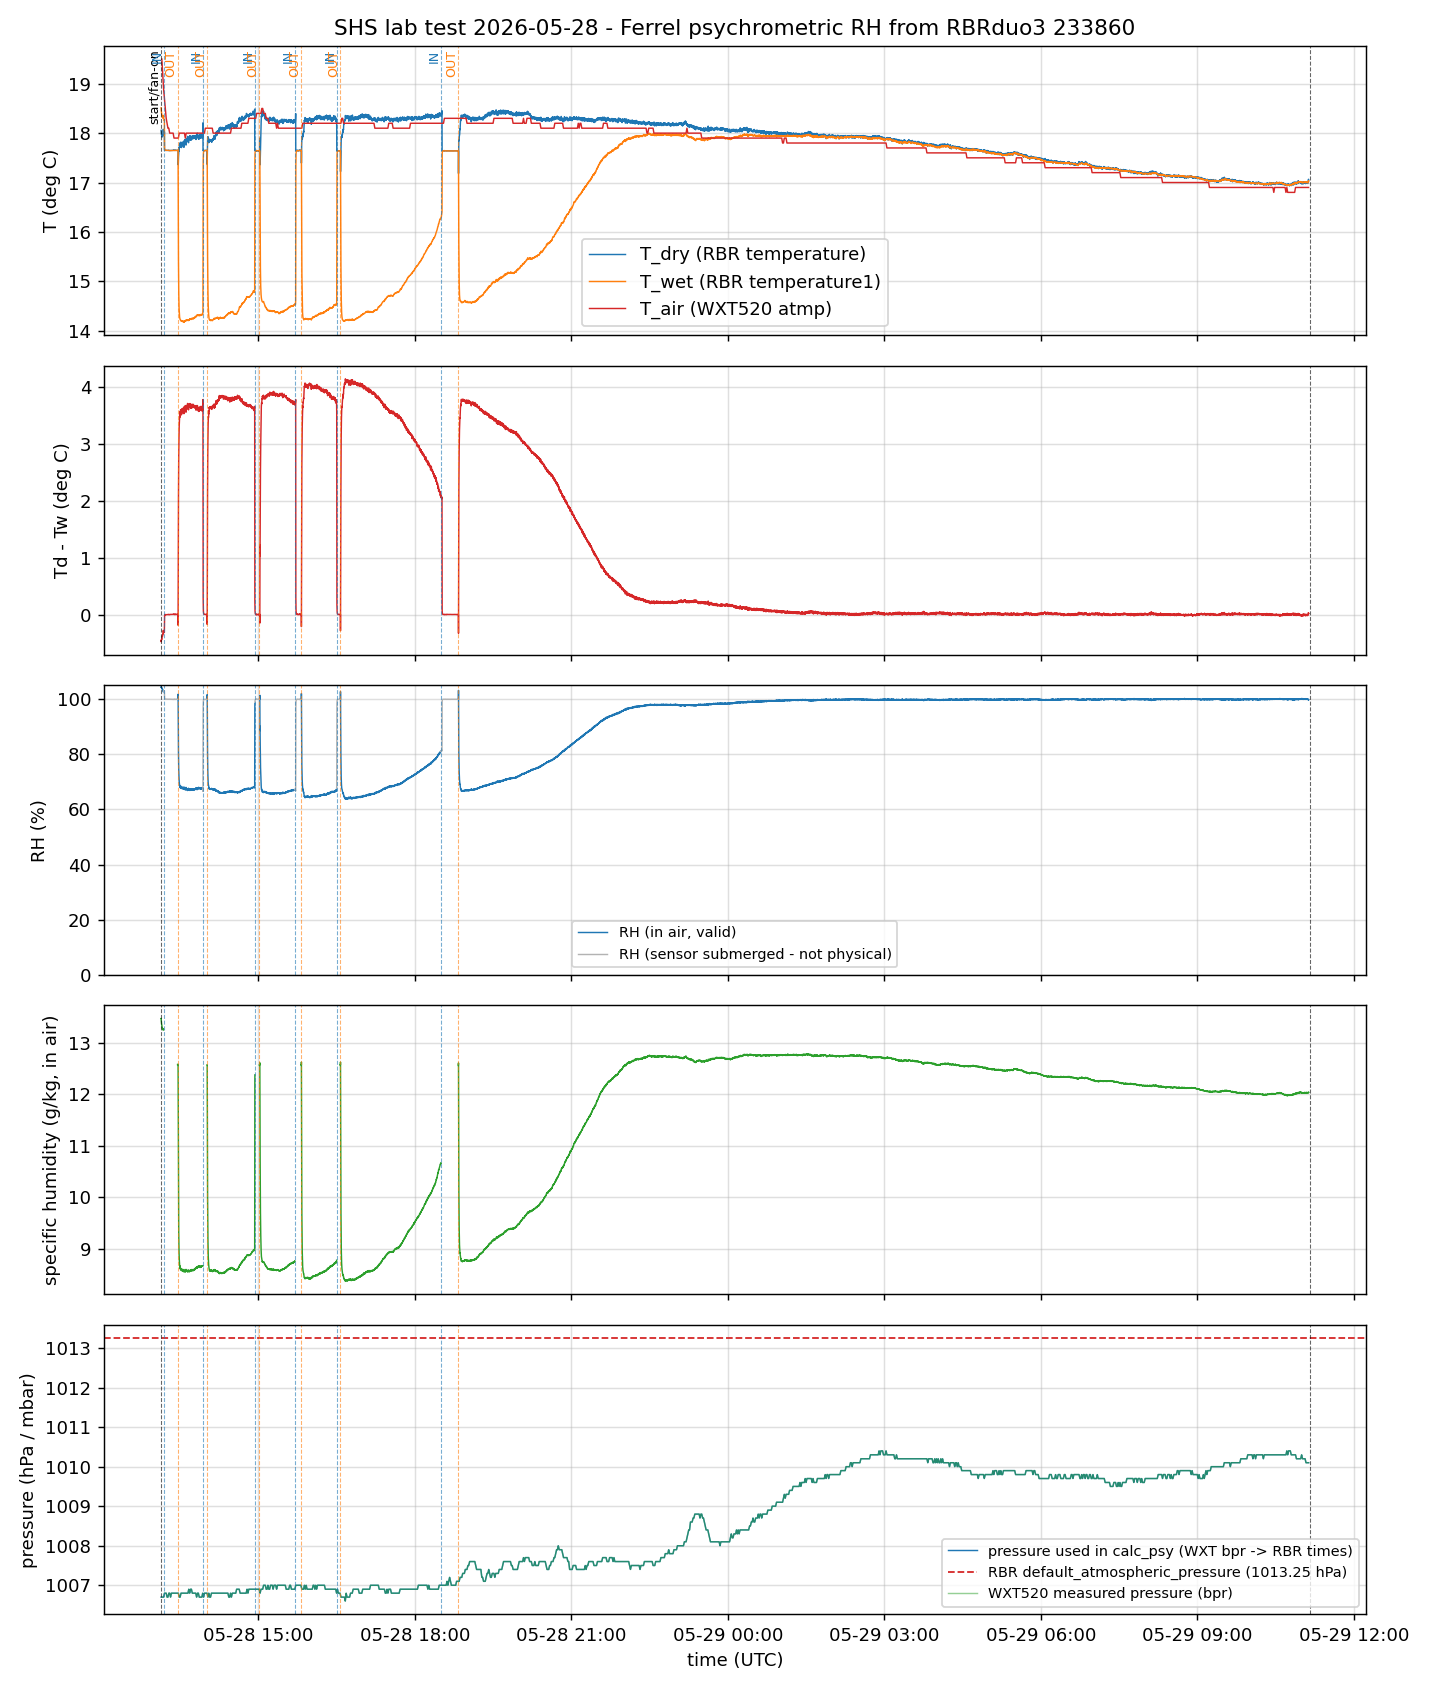
\includegraphics[width=\linewidth]{../../img/Lab20260528/Lab20260528_SHS_humidity.png}
  \caption{Psychrometric RH from SHS vs.\ WXT520 for all six dunk cycles.}
  \label{fig:shs_humidity}
\end{figure}

\begin{itemize}
  \item \textbf{IN-1 through IN-3:} Psychrometric RH undershoots the WXT
    reference.  Likely cause: wick not fully saturated at test start.
  \item \textbf{IN-4 onward:} Convergence to WXT RH ($\sim$64\,\%) once the
    wick is fully wetted.
  \item \textbf{Action item:} Add a live WXT display during the test for
    immediate feedback on wick saturation (per Simon's suggestion).
\end{itemize}

% ─────────────────────────────────────────────────────────────────────────────
\section{SHS vs.\ in-tank GPCTD reference}

\begin{figure}[htbp]
  \centering
  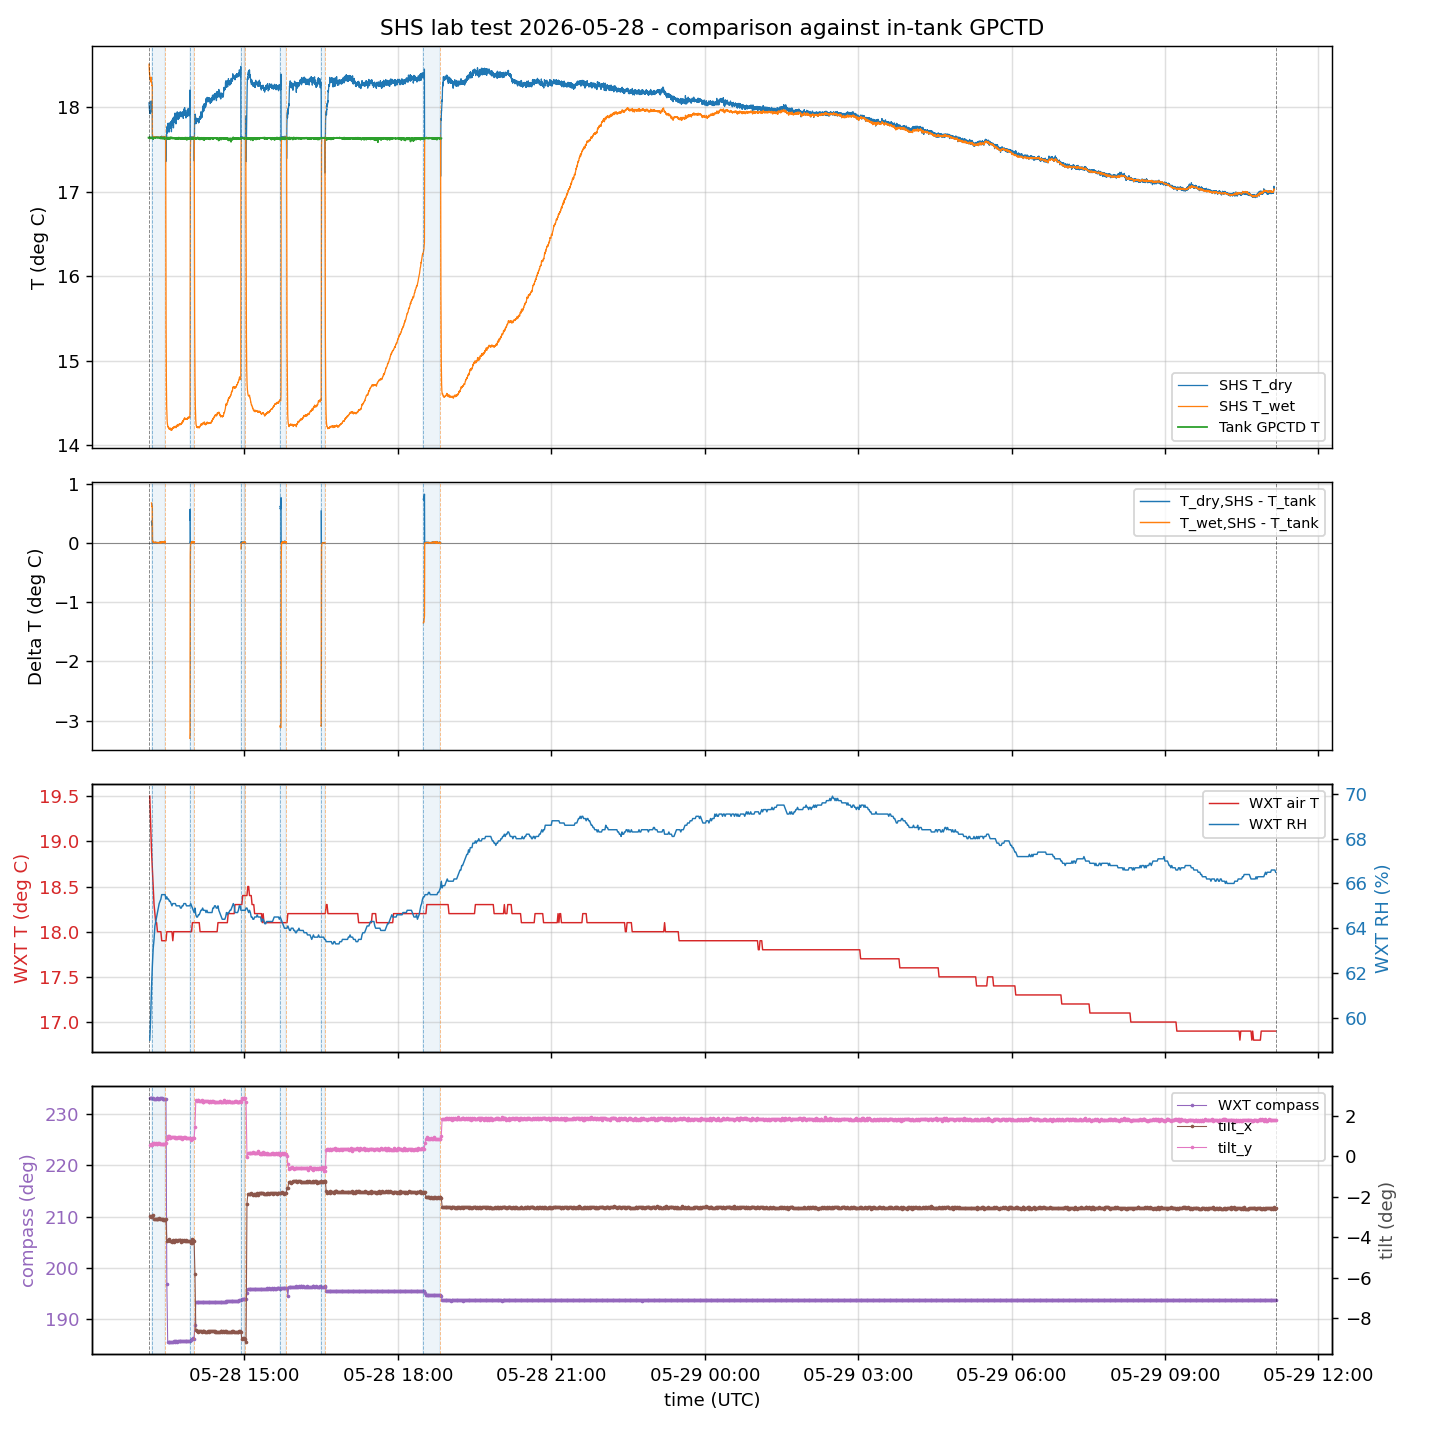
\includegraphics[width=\linewidth]{../../img/Lab20260528/Lab20260528_SHS_vs_tank.png}
  \caption{SHS temperatures vs.\ GPCTD tank reference during in-water periods.}
  \label{fig:vs_tank}
\end{figure}

$T_\text{wet}$ approaches tank temperature during each dunk;
$T_\text{dry}$ remains near ambient air due to its larger thermal mass.

% ─────────────────────────────────────────────────────────────────────────────
\section{Response times}

\textbf{Method.}
For each OUT event, a window is opened from the OUT time to
$\min(\text{OUT} + 25\,\text{min},\,\text{next IN})$.
The model
\begin{equation}
  y(t) = A + B\,e^{-t/\tau}
\end{equation}
is fitted by nonlinear least squares to $T_\text{dry}$, $T_\text{wet}$,
depression ($T_d - T_w$), and psychrometric RH independently, where $t=0$ at
the OUT time.  The time constant $\tau$ is the $e$-folding recovery time;
smaller $\tau$ means faster recovery.

\begin{center}
\begin{tabular}{lrrrr}
\toprule
OUT & $\tau_{T_d}$ (s) & $\tau_{T_w}$ (s) & $\tau_\text{dep}$ (s)
    & $\tau_\text{RH}$ (s) \\
\midrule
13:27 & 389  & 51 & 58 & 56 \\
14:01 & 1475$^*$ & 29 & 31 & 30 \\
15:01 &  74  & 61 & 65 & 64 \\
15:49 & 130  & 42 & 51 & 48 \\
16:34 & 139  & 41 & 54 & 51 \\
18:50 &  67  & 27 & 35 & 33 \\
\midrule
Median & 134 & 42 & 53 & 50 \\
\bottomrule
\end{tabular}

\smallskip{\footnotesize $^*$ window capped at 25 min; fit unreliable.}
\end{center}

See Figure~\ref{fig:response_time} for the individual fits.

$T_\text{wet}$, depression, and RH recover in $\sim$30--65\,s.
$T_\text{dry}$ is the slow component (median $\tau \approx 134$\,s); the
psychrometric RH inherits this slow recovery when computed through $T_\text{dry}$.

\begin{figure}[htbp]
  \centering
  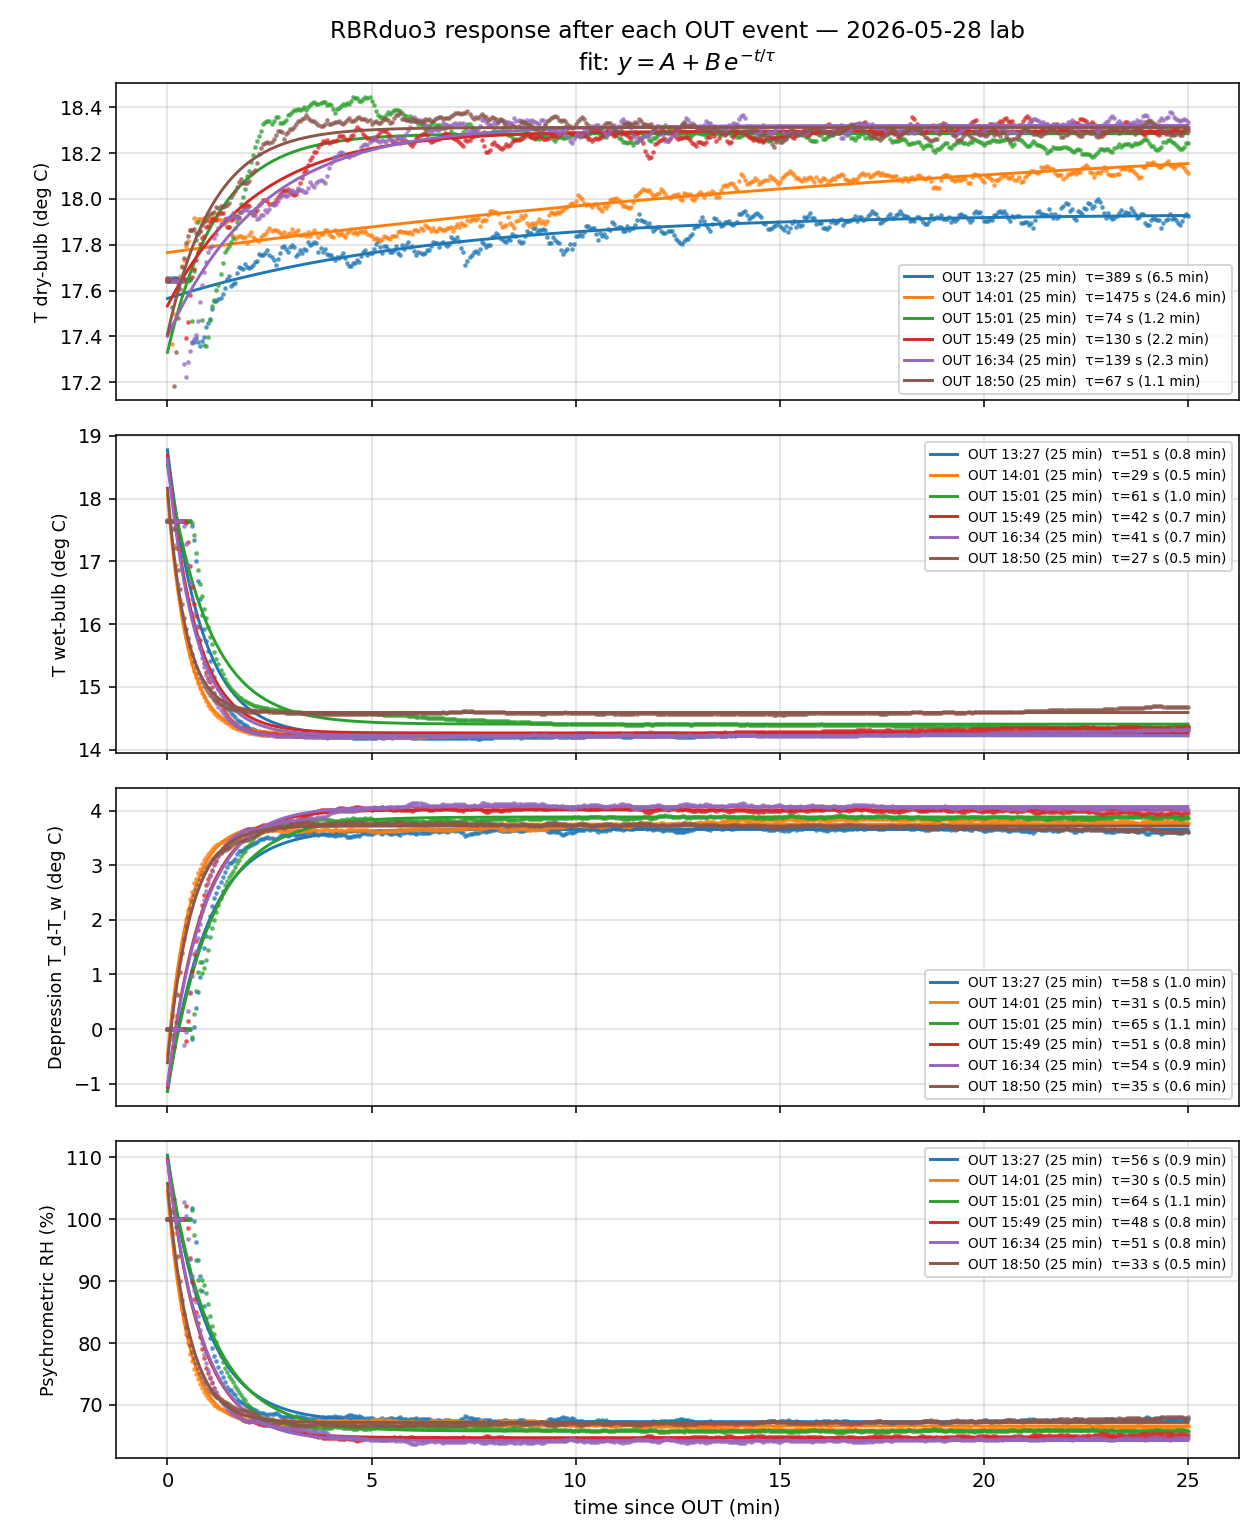
\includegraphics[width=\linewidth]{../../img/Lab20260528/Lab20260528_response_time.png}
  \caption{Exponential recovery fits for all six OUT events.}
  \label{fig:response_time}
\end{figure}

% ─────────────────────────────────────────────────────────────────────────────
\section{Wet-bulb cooling (IN events)}

\begin{figure}[htbp]
  \centering
  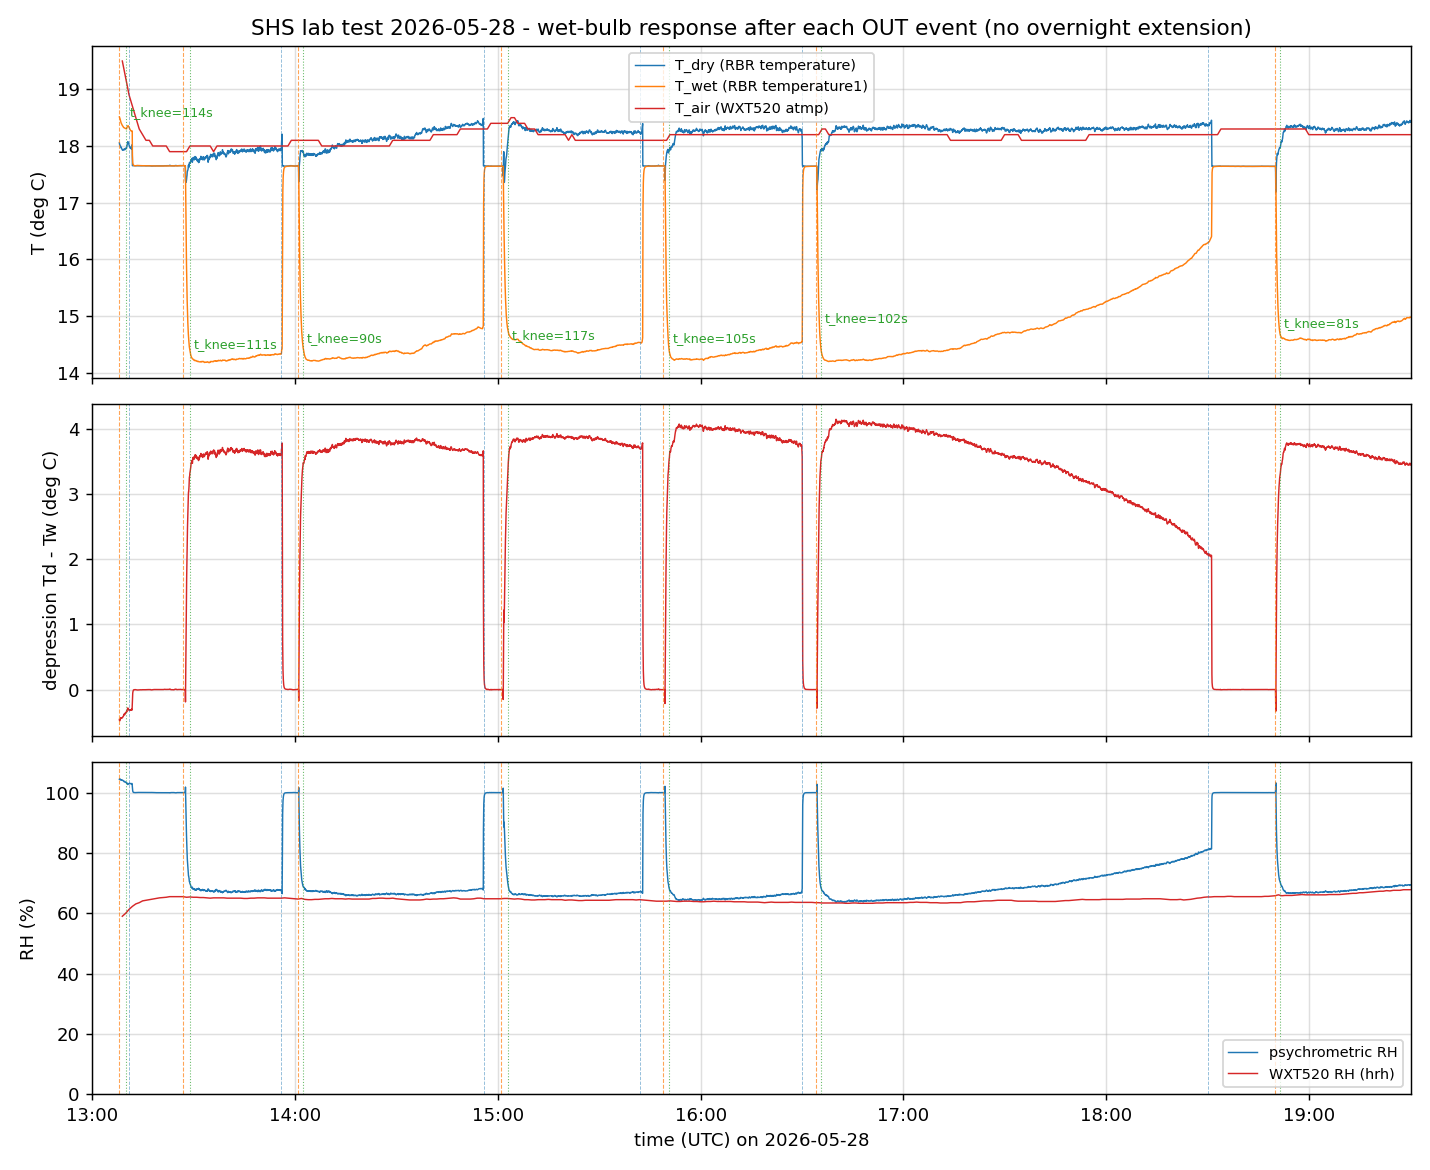
\includegraphics[width=\linewidth]{../../img/Lab20260528/Lab20260528_temp_drops.png}
  \caption{Wet-bulb cooling for each IN event.  Orange dashed line: OUT time.
           The sensor cools rapidly on submersion and plateaus near tank temperature.}
  \label{fig:temp_drops}
\end{figure}

$T_\text{wet}$ peaks in cooling rate at $\sim$20--50\,s after submersion and
reaches tank temperature within $\sim$1\,min.

% ─────────────────────────────────────────────────────────────────────────────
\section{Wind}

\begin{figure}[htbp]
  \centering
  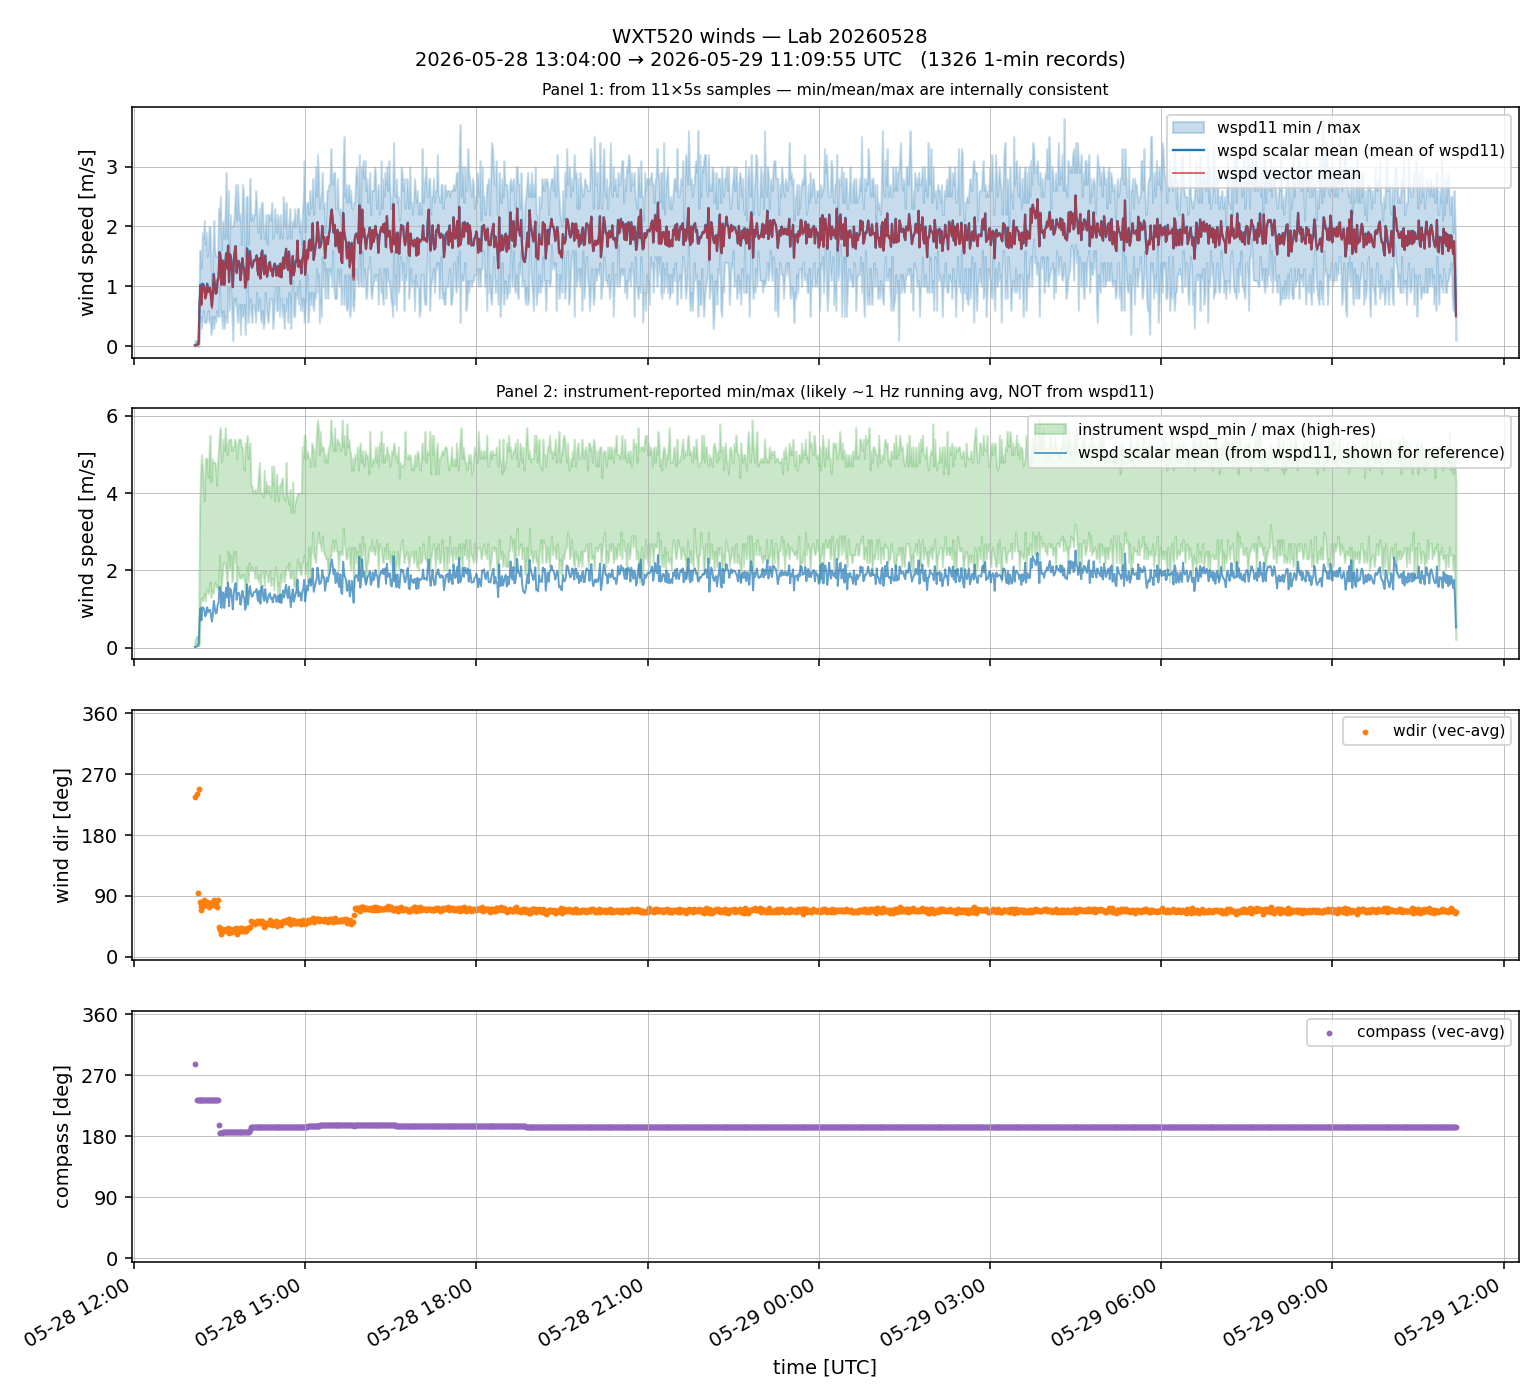
\includegraphics[width=\linewidth]{../../img/Lab20260528/WXT_wind_minmax_20260528.png}
  \caption{WXT520 wind.  \textbf{Top:} shaded band = min/max of \texttt{wspd11}
           (11 five-second samples/min); blue = scalar mean; red = vector mean.
           \textbf{Middle:} instrument-reported \texttt{wspd\_min}/\texttt{wspd\_max}
           (different population --- see text).
           \textbf{Bottom two:} wind direction and compass heading.}
  \label{fig:wind}
\end{figure}

Mean wind speed $\approx$1.8\,m/s (fan); compass stable at $\sim$195\si{\degree}.

\textbf{Note on \texttt{wspd\_min}/\texttt{wspd\_max}:}
The instrument stores these fields separately from the 11 archived samples.
The original MATLAB decoder labels \texttt{wspd11}-derived variables as
\emph{``of 11 samples''} but labels \texttt{wspd\_min}/\texttt{wspd\_max} only
as \emph{``for the minute''}, without further explanation.
\texttt{wspd\_min} exceeds \texttt{mean(wspd11)} in 99\,\% of records,
confirming they are not the min/max of \texttt{wspd11}.
All reported wind statistics use \texttt{wspd11} directly.
The Vaisala WXT520 manual is needed to clarify how these fields are computed
internally.

\end{document}
